
\documentclass[xcolor=dvipsnames]{beamer}  % for hardcopy add 'trans'

\mode<presentation>
{
  \usetheme{Singapore}
  % or ...
  \setbeamercovered{transparent}
  % or whatever (possibly just delete it)
}

\usefonttheme{professionalfonts}
%\usepackage[english]{babel}
% or whatever
%\usepackage[latin1]{inputenc}
% or whatever
%\usepackage{times}
%\usepackage[T1]{fontenc}
% Or whatever. Note that the encoding and the font should match. If T1
% does not look nice, try deleting the line with the fontenc.

%%%%%%%%%%%%%%%%%%%%%% start my preamble %%%%%%%%%%%%%%%%%%%%%%


\addtobeamertemplate{navigation symbols}{}{%
    \usebeamerfont{footline}%
    \usebeamercolor[fg]{footline}%
    \hspace{1em}%
    \insertframenumber/\inserttotalframenumber
}

\setbeamercolor{footline}{fg=blue}
\setbeamerfont{footline}{series=\bfseries}


%\usepackage{epsfig}
\usepackage{graphicx}
\usepackage{amsmath, amssymb, amsthm}

\usepackage{fancyvrb}

\usepackage{tikz}
\usetikzlibrary{arrows}
\usetikzlibrary{calc}
\usetikzlibrary{intersections}
\usetikzlibrary{decorations}
\usepackage{pgf}
\usepackage{pgfplots}
\pgfplotsset{compat=1.13}

\usepackage{graphviz}
 
\usepackage{verbatim}


\usepackage{algorithmicx,algpseudocode}


%font
\usepackage{mathpazo}
%\usepackage[usenames, dvipsnames]{color}

%\usepackage[linesnumbered, ruled, lined]{algorithm2e}

\usepackage{xr}
\externaldocument[ET-]{et}


\newcommand*{\theorembreak}{\usebeamertemplate{theorem end}\framebreak\usebeamertemplate{theorem begin}}

\newcommand{\newtopic}[1]{\textcolor{Green}{\Large \bf #1}}
\newcommand{\navy}[1]{\textcolor{Blue}{\bf #1}}
\newcommand{\navymth}[1]{\textcolor{Blue}{#1}}
\newcommand{\red}[1]{\textcolor{red}{#1}}


\definecolor{pale}{RGB}{235, 235, 235}
\definecolor{pale2}{RGB}{175,238,238}
\definecolor{turquois4}{RGB}{0,134,139}

% Typesetting code
\definecolor{bg}{rgb}{0.95,0.95,0.95}
\usepackage{minted}
\usemintedstyle{friendly}
\newminted{python}{mathescape,frame=lines,framesep=4mm,bgcolor=bg}
\newminted{ipython}{mathescape,frame=lines,framesep=4mm,bgcolor=bg}
\newminted{julia}{mathescape,frame=lines,framesep=4mm,bgcolor=bg}
\newminted{c}{mathescape,linenos=true}
\newminted{r}{mathescape,  frame=none, baselinestretch=1, framesep=2mm}
\renewcommand{\theFancyVerbLine}{\sffamily
    \textcolor[rgb]{0.5,0.5,1.0}{\scriptsize {\arabic{FancyVerbLine}}}}


\usepackage{stmaryrd}

\newcommand{\Fact}{\textcolor{Brown}{\bf Fact. }}
\newcommand{\Facts}{\textcolor{Brown}{\bf Facts }}
\newcommand{\keya}{\textcolor{turquois4}{\bf Key Idea. }}
\newcommand{\Factnodot}{\textcolor{Brown}{\bf Fact }}
\newcommand{\Eg}{\textcolor{ForestGreen}{Example. }}
\newcommand{\Egs}{\textcolor{ForestGreen}{Examples. }}
\newcommand{\Ex}{{\bf Ex. }}
\newcommand{\Thm}{\textcolor{Brown}{\bf Theorem. }}
\newcommand{\Prf}{\textcolor{turquois4}{\bf Proof.}}
\newcommand{\Ass}{\textcolor{turquois4}{\bf Assumption.}} 
\newcommand{\Lem}{\textcolor{Brown}{\bf Lemma. }}

%source code 



% caligraphic
\usepackage{mathrsfs}
\usepackage{bbm}
\usepackage{subfigure}

\newcommand{\argmax}{\operatornamewithlimits{argmax}}
\newcommand{\argmin}{\operatornamewithlimits{argmin}}

\newcommand\T{{\mathpalette\raiseT\intercal}}
\newcommand\raiseT[2]{\raisebox{0.25ex}{$#1#2$}}

\DeclareMathOperator{\cl}{cl}
%\DeclareMathOperator{\argmax}{argmax}
\DeclareMathOperator{\interior}{int}
\DeclareMathOperator{\Prob}{Prob}
\DeclareMathOperator{\kernel}{ker}
\DeclareMathOperator{\diag}{diag}
\DeclareMathOperator{\sgn}{sgn}
\DeclareMathOperator{\determinant}{det}
\DeclareMathOperator{\trace}{trace}
\DeclareMathOperator{\Span}{span}
\DeclareMathOperator{\rank}{rank}
\DeclareMathOperator{\cov}{cov}
\DeclareMathOperator{\corr}{corr}
\DeclareMathOperator{\range}{rng}
\DeclareMathOperator{\var}{var}
\DeclareMathOperator{\mse}{mse}
\DeclareMathOperator{\se}{se}
\DeclareMathOperator{\row}{row}
\DeclareMathOperator{\col}{col}
\DeclareMathOperator{\dimension}{dim}
\DeclareMathOperator{\fracpart}{frac}
\DeclareMathOperator{\proj}{proj}
\DeclareMathOperator{\colspace}{colspace}

\providecommand{\inner}[1]{\left\langle{#1}\right\rangle}

% mics short cuts and symbols
% mics short cuts and symbols
\newcommand{\st}{\ensuremath{\ \mathrm{s.t.}\ }}
\newcommand{\setntn}[2]{ \{ #1 : #2 \} }
\newcommand{\cf}[1]{ \lstinline|#1| }
\newcommand{\otms}[1]{ \leftidx{^\circ}{#1}}

\newcommand{\fore}{\therefore \quad}
\newcommand{\tod}{\stackrel { d } {\to} }
\newcommand{\tow}{\stackrel { w } {\to} }
\newcommand{\toprob}{\stackrel { p } {\to} }
\newcommand{\toms}{\stackrel { ms } {\to} }
\newcommand{\eqdist}{\stackrel {\textrm{ \scriptsize{d} }} {=} }
\newcommand{\iidsim}{\stackrel {\textrm{ {\sc iid }}} {\sim} }
\newcommand{\1}{\mathbbm 1}
\newcommand{\dee}{\,{\rm d}}
\newcommand{\given}{\, | \,}
\newcommand{\la}{\langle}
\newcommand{\ra}{\rangle}

\renewcommand{\rho}{\varrho}

\newcommand{\htau}{ \hat \tau }
\newcommand{\hgamma}{ \hat \gamma }

\newcommand{\boldx}{ {\mathbf x} }
\newcommand{\boldu}{ {\mathbf u} }
\newcommand{\boldv}{ {\mathbf v} }
\newcommand{\boldw}{ {\mathbf w} }
\newcommand{\boldy}{ {\mathbf y} }
\newcommand{\boldb}{ {\mathbf b} }
\newcommand{\bolda}{ {\mathbf a} }
\newcommand{\boldc}{ {\mathbf c} }
\newcommand{\boldi}{ {\mathbf i} }
\newcommand{\bolde}{ {\mathbf e} }
\newcommand{\boldp}{ {\mathbf p} }
\newcommand{\boldq}{ {\mathbf q} }
\newcommand{\bolds}{ {\mathbf s} }
\newcommand{\boldt}{ {\mathbf t} }
\newcommand{\boldz}{ {\mathbf z} }

\newcommand{\boldzero}{ {\mathbf 0} }
\newcommand{\boldone}{ {\mathbf 1} }

\newcommand{\boldalpha}{ {\boldsymbol \alpha} }
\newcommand{\boldbeta}{ {\boldsymbol \beta} }
\newcommand{\boldgamma}{ {\boldsymbol \gamma} }
\newcommand{\boldtheta}{ {\boldsymbol \theta} }
\newcommand{\boldxi}{ {\boldsymbol \xi} }
\newcommand{\boldtau}{ {\boldsymbol \tau} }
\newcommand{\boldepsilon}{ {\boldsymbol \epsilon} }
\newcommand{\boldmu}{ {\boldsymbol \mu} }
\newcommand{\boldSigma}{ {\boldsymbol \Sigma} }
\newcommand{\boldOmega}{ {\boldsymbol \Omega} }
\newcommand{\boldPhi}{ {\boldsymbol \Phi} }
\newcommand{\boldLambda}{ {\boldsymbol \Lambda} }
\newcommand{\boldphi}{ {\boldsymbol \phi} }

\newcommand{\Sigmax}{ {\boldsymbol \Sigma_{\boldx}}}
\newcommand{\Sigmau}{ {\boldsymbol \Sigma_{\boldu}}}
\newcommand{\Sigmaxinv}{ {\boldsymbol \Sigma_{\boldx}^{-1}}}
\newcommand{\Sigmav}{ {\boldsymbol \Sigma_{\boldv \boldv}}}

\newcommand{\hboldx}{ \hat {\mathbf x} }
\newcommand{\hboldy}{ \hat {\mathbf y} }
\newcommand{\hboldb}{ \hat {\mathbf b} }
\newcommand{\hboldu}{ \hat {\mathbf u} }
\newcommand{\hboldtheta}{ \hat {\boldsymbol \theta} }
\newcommand{\hboldtau}{ \hat {\boldsymbol \tau} }
\newcommand{\hboldmu}{ \hat {\boldsymbol \mu} }
\newcommand{\hboldbeta}{ \hat {\boldsymbol \beta} }
\newcommand{\hboldgamma}{ \hat {\boldsymbol \gamma} }
\newcommand{\hboldSigma}{ \hat {\boldsymbol \Sigma} }

\newcommand{\boldA}{\mathbf A}
\newcommand{\boldB}{\mathbf B}
\newcommand{\boldC}{\mathbf C}
\newcommand{\boldD}{\mathbf D}
\newcommand{\boldI}{\mathbf I}
\newcommand{\boldL}{\mathbf L}
\newcommand{\boldM}{\mathbf M}
\newcommand{\boldP}{\mathbf P}
\newcommand{\boldQ}{\mathbf Q}
\newcommand{\boldR}{\mathbf R}
\newcommand{\boldX}{\mathbf X}
\newcommand{\boldU}{\mathbf U}
\newcommand{\boldV}{\mathbf V}
\newcommand{\boldW}{\mathbf W}
\newcommand{\boldY}{\mathbf Y}
\newcommand{\boldZ}{\mathbf Z}

\newcommand{\bSigmaX}{ {\boldsymbol \Sigma_{\hboldbeta}} }
\newcommand{\hbSigmaX}{ \mathbf{\hat \Sigma_{\hboldbeta}} }

\newcommand{\RR}{\mathbbm R}
\newcommand{\CC}{\mathbbm C}
\newcommand{\NN}{\mathbbm N}
\newcommand{\PP}{\mathbbm P}
\newcommand{\EE}{\mathbbm E \nobreak\hspace{.1em}}
\newcommand{\EEP}{\mathbbm E_P \nobreak\hspace{.1em}}
\newcommand{\ZZ}{\mathbbm Z}
\newcommand{\QQ}{\mathbbm Q}


\newcommand{\XX}{\mathcal X}

\newcommand{\aA}{\mathcal A}
\newcommand{\fF}{\mathscr F}
\newcommand{\bB}{\mathscr B}
\newcommand{\iI}{\mathscr I}
\newcommand{\rR}{\mathscr R}
\newcommand{\dD}{\mathcal D}
\newcommand{\lL}{\mathcal L}
\newcommand{\llL}{\mathcal{H}_{\ell}}
\newcommand{\gG}{\mathcal G}
\newcommand{\hH}{\mathcal H}
\newcommand{\nN}{\textrm{\sc n}}
\newcommand{\lN}{\textrm{\sc ln}}
\newcommand{\pP}{\mathscr P}
\newcommand{\qQ}{\mathscr Q}
\newcommand{\xX}{\mathcal X}

\newcommand{\ddD}{\mathscr D}


\newcommand{\R}{{\texttt R}}
\newcommand{\risk}{\mathcal R}
\newcommand{\Remp}{R_{{\rm emp}}}

\newcommand*\diff{\mathop{}\!\mathrm{d}}
\newcommand{\ess}{ \textrm{{\sc ess}} }
\newcommand{\tss}{ \textrm{{\sc tss}} }
\newcommand{\rss}{ \textrm{{\sc rss}} }
\newcommand{\rssr}{ \textrm{{\sc rssr}} }
\newcommand{\ussr}{ \textrm{{\sc ussr}} }
\newcommand{\zdata}{\mathbf{z}_{\mathcal D}}
\newcommand{\Pdata}{P_{\mathcal D}}
\newcommand{\Pdatatheta}{P^{\mathcal D}_{\theta}}
\newcommand{\Zdata}{Z_{\mathcal D}}




\newcommand{\e}[1]{\mathbbm{E}[{#1}]}
\newcommand{\p}[1]{\mathbbm{P}({#1})}

%\theoremstyle{plain}
%\newtheorem{axiom}{Axiom}[section]
%\newtheorem{theorem}{Theorem}[section]
%\newtheorem{corollary}{Corollary}[section]
%\newtheorem{lemma}{Lemma}[section]
%\newtheorem{proposition}{Proposition}[section]
%
%\theoremstyle{definition}
%\newtheorem{definition}{Definition}[section]
%\newtheorem{example}{Example}[section]
%\newtheorem{remark}{Remark}[section]
%\newtheorem{notation}{Notation}[section]
%\newtheorem{assumption}{Assumption}[section]
%\newtheorem{condition}{Condition}[section]
%\newtheorem{exercise}{Ex.}[section]
%\newtheorem{fact}{Fact}[section]

% Bibliography
\usepackage[authordate,uniquename=false,firstinits,backend=biber,maxcitenames=2]{biblatex-chicago}
\DeclareFieldFormat[article]{title}{#1}
\DeclareFieldFormat[inproceedings]{title}{#1}
\addbibresource{et_newbib.bib}
\renewcommand{\cite}{\textcite}



\setlength{\parskip}{1.5ex plus0.5ex minus0.5ex}


\setlength{\jot}{12pt} 








\title{A Primer in Econometric Theory}

\subtitle
{Lecture 7: Estimators}

\author{John Stachurski \\ \tiny Lectures by Akshay Shanker}


\begin{document}

\begin{frame}
  \titlepage
\end{frame}

\section{The Estimation Problem}

\begin{frame}\frametitle{Probability and Statistics}
    
    \vspace{2em}
    Probability theory
        \begin{itemize}
            \item aim to deduce the likelihood of different
        outcomes based on known probability distributions
        \end{itemize}
    
    \vspace{.7em}    
    Statistics
        \begin{itemize}
            \item infer unknown probability distributions from outcomes we
            observe
        \end{itemize}

\end{frame}

\begin{frame}
    
    \vspace{2em}
    Start in setting where successive observations are {\sc iid}
    
    \vspace{.7em}
    The fundamental problem of econometrics and statistics:
    
    \begin{problem}
        We observe independent $Z$-valued draws $\boldz_1, \ldots, \boldz_N$ 
        from a common but
        unknown distribution $P \in \pP$, where $\pP$ is a class of distributions
        on $Z$.   We wish to infer some features of $P$ from this sample.
    \end{problem}
    
\end{frame}

\begin{frame}

    \vspace{2em}
    The set $\pP$ can be anything, including the set of all distributions 
    on the outcome space
    
    \vspace{.7em}
    A task of economic theory is to restrict $\pP$ narrow the set of 
    distributions to search over
    
    \vspace{.7em}
    \Eg
    \cite{benhabib2015wealth} study the wealth distribution in a model with
    idiosyncratic capital income risk
    
    The model predicts that the wealth
    distribution will have a Pareto right tail
    
\end{frame}

\begin{frame}
    
    \vspace{2em}
    Some notation:
    %
    \begin{itemize}
        \label{enum:sen}
        \item $Z$ is the \navy{outcome space} where each \navy{observation}
            $\boldz_n$ takes values
        \item $\zdata$ denotes the \navy{sample} or \navy{data set} $(\boldz_1, \ldots,
            \boldz_N)$
        \item $\Zdata := \times_{n=1}^N Z$ is the \navy{sample space} 
            in which $\zdata$ takes values
        \item $\Pdata := \lL(\zdata)$ is the \navy{joint distribution of the
            sample}
    \end{itemize}
    
    Note calling $\Zdata$ the sample space is overloading terminology 
    used to describe probability spaces 
    
    \vspace{.7em}
    Assume {\sc iid} data, so the joint distribution
    $\Pdata$ will be the $N$th product of $P$


\end{frame}


\begin{frame}
    
    \vspace{2em}
    \Eg
    Let $x_1, \ldots, x_N$ be observations of labor
    income from a given population
    
    We model $x_1, \ldots, x_N$ as {\sc iid}
    draws from a common univariate distribution $P$
    
    In our terminology:
    %
    \begin{itemize}
        \item $x_n$ is an observation
        \item the outcome space $Z$ is
                $\RR$
        \item the sample space $\Zdata$ is $\RR^N$
        \item the sample $\zdata$ is the vector $(x_1, \ldots, x_N)$
    \end{itemize}
    
\end{frame}

\begin{frame}
    
    \vspace{2em}
    Features of $P$ we might wish to
    learn about:

    \begin{itemize}
        \item the mean and higher moments of $P$,
        \item measures of dispersion, such as the variance, or properties of
            tails,
        \item the median and other quantiles, and
        \item $P$ itself, or the density of $P$ if it exists
    \end{itemize}
\end{frame}

\begin{frame}
    
    \vspace{2em}
    \Eg
    Suppose we wish to learn about the relationship between profitability and
    R\&D spending within a group of firms
    
    Let $\boldz_n = (x_n, y_n)$ be an
    observation of these two quantities at the $n$th firm
    
    \vspace{.7em}
    Treat the
    observations as {\sc iid} across firms, with common marginal distribution $P =
    \lL(\boldz_n)$
    
    The outcome space is $Z = \RR^2$, and the sample space:
    %
    \begin{equation*}
        \Zdata := \RR^2 \times \cdots \times \RR^2 = \RR^{2 \times N}
    \end{equation*}
    
\end{frame}

\begin{frame}
    
    \vspace{2em}
    Marginal distribution $P$ of the observations is now
    multivariate -- new features:
    %
    \begin{itemize}
        \item correlations across coordinates of $P$,
        \item the variance--covariance matrix associated with $P$, and
        \item parameters controlling dependence when, say, $P$ is modeled via a copula over certain marginals
    \end{itemize}
    
\end{frame}

\begin{frame}\frametitle{Features of P}
    
    \vspace{2em}
    Define a \navy{feature} of $P$ to be an
    object of the form
    %
    \begin{equation*}
        \label{eq:dfeature}
        \gamma(P)
        \quad \text{for some} \quad
        \gamma \colon \pP \to S
    \end{equation*}
    
    \vspace{1em}
    When $P$ is understood, we'll write $\gamma(P)$ as $\gamma$
    
\end{frame}

\begin{frame}
    
    \vspace{2em}
    Examples for univariate $P$
    routinely estimated in econometric studies:  
    
    \begin{itemize}
        \item $\gamma(P) = \int s^k P(\diff s)$, the $k$th moment of $P$
        \item $\gamma(P) = \inf\setntn{s \in \RR}{P(- \infty, s] \geq 1/2}$, the
            median of $P$
        \item $\gamma(P) = P$, when we want to estimate $P$ itself
        \item $\gamma(P) = $ the density of $P$ when $P$ is absolutely continuous
    \end{itemize}
      
    \vspace{.7em}
    If $P$ is multivariate over $\boldz = (\boldx, y)$, then a feature of interest is the regression function
    $f^*(\boldx) := \EE[ y \given \boldx]$
    \begin{itemize}
        \item the function is uniquely determined by $P$ (recall our discussion in \S\ref{ET-ss:ce})
    \end{itemize}
    
\end{frame}

\begin{frame}\frametitle{Parametric and Nonparametric Classes}
    
    \vspace{2em}
    We assumed above that the unknown distribution belongs to some class $\mathscr{P}$ 
    
    \vspace{.7em}
    A  class of distributions is called a \navy{parametric class} if it can be indexed by
    finitely many parameters
    %
    \begin{equation*}
        \pP = \{P_{\boldtheta}\}_{\boldtheta \in \Theta} :=:
        \setntn{P_{\boldtheta}}{\boldtheta \in \Theta}
        \quad \text{for some } \Theta \subset \RR^K
    \end{equation*}
    %
    A class of distributions is called
    \navy{nonparametric} if it is not parametric
    
\end{frame}

\begin{frame}
    
    \vspace{2em}
    \Eg
    Let $\pP$ be the set of 
    all univariate normal distributions with positive variance:
    %
    \begin{align*}
        \pP := 
        \bigg\{
        \text{all } p \; \st \;
        p(s) = \frac{1}{\sqrt{2 \pi} \sigma}
       \exp \left\{ - \frac{(s - \mu)^2}{2\sigma^2} \right\}
       \; \\ \text{ for some }
       \; \mu \in \RR, \; \sigma > 0
       \bigg\}
    \end{align*}
    
    The set $\pP$ is an example of a parametric class
    
    \begin{itemize}
        \item the parameters
    are $\boldtheta = (\mu, \sigma)$
        \item particular choice of parameters
    determines (parameterizes) an element of the class
    \end{itemize}
    
\end{frame}

\begin{frame}

    \vspace{2em}
    \Eg
    Suppose outcome space $Z$ is finite, containing $J$ elements
    
    Every distribution $P$ on $Z$ can be represented by $J-1$ parameters (the
    probability $p_j$ of each outcome but the last) 
    
    Hence any family $\pP$
    of distributions on $Z$ is a parametric class
  
    \vspace{.7em}
    \Eg
    The set of all distributions on $\RR$ cannot be parameterized by a
    finite vector of parameters because the space of distributions is infinite
    dimensional
    
    Hence $\pP :=$ all distributions on $\RR$ is a
    nonparametric class
    
\end{frame}

\begin{frame}
    
    \vspace{2em}
    \Eg
    Let $\pP$ be the set of all absolutely continuous distributions on $\RR$
    with finite second moment:
    %
    \small \begin{equation*}
        \pP := \left\{\text{all} p \colon \RR \to \RR \st
        p \geq 0, \; \int p(s)\diff s = 1, \; \int s^2 p(s) \diff s < \infty \right\}
    \end{equation*}
    %
    The set is ....
    
\end{frame}

\begin{frame}
    
    \vspace{2em}
    Traditional methods of inference:
    
    \begin{itemize}
        \item  assume data generated by an unknown element $P_{\boldtheta}$ of a
        parametric class $\pP$
        \item estimate $\boldtheta$ using the data  -- the estimate of $\boldtheta$ is $\hboldtheta$ 
        \item plug $\hboldtheta$ back into
        the parametric class to obtain an estimate $P_{\hboldtheta}$ of $P_{\boldtheta}$
    \end{itemize}
    
\end{frame}

\begin{frame}
    
    \vspace{2em}
    In parametric settings, the feature $\gamma$ that we are most interested
    in estimating is the parameter vector $\boldtheta$
    
    \vspace{.7em}
    If we have a good estimate
    $\hboldtheta$ of $\boldtheta$, we can estimate any feature $\gamma =
    \gamma(P_{\boldtheta})$ via $\hat \gamma = \gamma(P_{\hboldtheta})$
    
\end{frame}

\begin{frame}
    
    \vspace{2em}
    Common usage -- refer to the $\boldtheta$ associated
    with the $P_\boldtheta$ that generates the data as the \navy{true value} of
    the parameter vector
    \begin{itemize}
    \item  an assumption, not a ``truth."!
    \end{itemize}
    
    We \emph{assume} data generated by
    some member of a parametric class
    
    Assumption can be completely false
    
\end{frame}

\begin{frame}
    
    \vspace{2em}
    Why did we first formulate the problem as estimation of features?
    \begin{itemize}
        \item because it is suboptimal to always
        restrict ourselves to parametric assumptions on $\pP$
    \end{itemize}
    
    Discussion of relative merits of parametric and 
    nonparametric estimation in chapter~\ref{ET-c:rms}
    
\end{frame}

\begin{frame}\frametitle{Statistics and Estimators}
    
    \vspace{2em}
    A \navy{statistic} is any $\bB$-measurable function 
    %
    \begin{equation*}
        T \colon \Zdata \to S
    \end{equation*}
    %
    that can be evaluated once the data $\zdata$ are observed
    
    \vspace{.7em}
    As in \eqref{eq:dfeature}, the
    set $S$ is left arbitrary to accommodate all the possible features that we
    might wish to estimate
    
    Sometimes write $T$ as $T_N$ to emphasize
    dependence on the sample size
    
\end{frame}

\begin{frame}
    
    \vspace{2em}
    An \navy{estimator} is a statistic used to
    infer some feature $\gamma(P)$ of an unknown distribution $P$\
    \begin{itemize}
        \item statistic becomes an estimator when paired with and
        compared to a feature of
    the distribution
    \end{itemize}
    
    \vspace{.7em}
    Nothing in the definition of an
    estimator that implies it will be a good estimator of the target feature
    
\end{frame}

\begin{frame}

    \vspace{2em}
    \Eg
    If the feature $\gamma$ we wish to infer is the mean of the marginal
    distribution $P$ of {\sc iid} data $x_1, \ldots, x_N$, then
    the most common estimator is the \navy{sample mean}
    %
    \begin{equation*}
        \bar x_N := \frac{1}{N} \sum_{n=1}^N x_n
    \end{equation*}
    %
    Formally, $\bar x_N$ is the mapping from $\Zdata = \RR^N$ to $S = \RR$
    defined by 
    %
    \begin{equation*}
     \zdata = (x_1, \ldots, x_N)
        \mapsto
        T(x_1, \ldots, x_N)
        = \frac{1}{N} \sum_{n=1}^N x_n  \in \RR
    \end{equation*}
    %
    This mapping is regarded as an estimator of the unknown mean $\gamma(P) =
    \int s P(\diff s)$
    
\end{frame}

\begin{frame}
    
    \vspace{2em}
    \Eg
    The sample mean is not the only way to estimate the mean. For example, we
    could also use the so-called \navy{mid-range estimator}
    %
    \begin{equation*}
        m_N := \frac{\min_n x_n + \max_n x_n }{2}
    \end{equation*}
    
    \vspace{2em}
    Another option is a \navy{truncated sample mean}, where values $x_n$ with
    $|x_n| \geq r$ are truncated for some specified value of $r$.  The
    truncated sample mean is often used to estimate location parameters in
    heavy tailed distributions
\end{frame}

\begin{frame}

    \vspace{2em}
    \Eg
    Given sample $x_1, \ldots, x_N$, let $y_n$ be the $n$th
    largest observation of the sample.  If $N$ is the odd number $2m+1$,
    the \navy{sample median} is defined as $y_{m+1}$.  If $N=2m$,
    the sample median is $0.5(y_m + y_{m+1})$.
        
    \vspace{.7em}    
    \Eg
    A common estimator of the $k$th
    moment $\int s^k P(\diff s)$ of $P$ is the $k$th \navy{sample moment}
    $\frac{1}{N} \sum_{n=1}^N x_n^k$.

\end{frame}

\begin{frame}

    \vspace{2em}
    \Eg
    A common estimator of the variance of $P$  is the \navy{sample
        variance}
    %
    \begin{equation*}
        \label{eq:sampvar}
        s_N^2 := \frac{1}{N} \sum_{n=1}^N (x_n - \bar x_N)^2
    \end{equation*}
    
    \vspace{.7em}
    The standard deviation is usually estimated using \navy{sample standard deviation} 
    %
    \begin{equation*}
        \label{eq:sampsd}
        s_N 
        := \sqrt{s^2_N} 
        = \left[ 
            \frac{1}{N} \sum_{n=1}^N (x_n - \bar x_N)^2
            \right]^{1/2}
    \end{equation*}
    
\end{frame}

\begin{frame}
    
    \vspace{2em}
    \Eg
    Given bivariate data $\zdata = ((x_1, y_1), \ldots, (x_N, y_N))$,
    the \navy{sample covariance} is the statistic
    %
    \begin{equation*}
        \label{eq:sampcov}
        \frac{1}{N} \sum_{n=1}^N (x_n - \bar x_N)(y_n - \bar y_N)
    \end{equation*}
    
    \vspace{.7em}
    The \navy{sample correlation} is the sample covariance divided by the 
    product of the two sample standard deviations.  With some rearranging, this becomes
    %
    \begin{equation*}
        \label{eq:sampcorr}
        \frac{\sum_{n=1}^N (x_n - \bar x_N)(y_n - \bar y_N)}
        { 
        \sqrt{ \sum_{n=1}^N (x_n - \bar x_N)^2 \sum_{n=1}^N (y_n - \bar y_N)^2 }
        }
    \end{equation*}
    
\end{frame}

\begin{frame}
    
    \vspace{2em}
    \Eg
    In the case where our observations are vectors $\boldx_1,\ldots,\boldx_N$ in
    $\RR^K$, the sample mean is the random vector defined by
    %
    \begin{equation*}
        \bar \boldx_N := \frac{1}{N} \sum_{n=1}^N \boldx_n 
    \end{equation*}
    %
    The variance--covariance matrix is most often
    estimated with the \navy{sample variance--covariance matrix} 
    %
    \begin{equation*}
        \hboldSigma_N := \frac{1}{N} \sum_{n=1}^N 
            [ (\boldx_n - \bar \boldx_N) (\boldx_n - \bar \boldx_N)^\T]
    \end{equation*}
    
\end{frame}

\section{Empirical Distribution}

\begin{frame}\frametitle{Empirical Distribution}

    \vspace{2em}
    The \navy{empirical distribution} of a given $Z$-valued sample $\zdata = (\boldz_1,
    \ldots, \boldz_N)$ is the discrete distribution on $Z$ that puts equal
    probability $1/N$ on each sample point $\boldz_n$
    
    \vspace{.7em}
    $\hat P_N$ assigns to each Borel set $B \subset Z$ 
    the number
    %
    \begin{equation*}
        \label{eq:dempd}
        \hat P_N(B) = \frac{1}{N} \sum_{n=1}^N \1\{\boldz_n \in B\}
    \end{equation*}
    %
    This is just the fraction of the sample that falls in $B$
    
\end{frame}

\begin{frame}
    
    \vspace{2em}
    The expectation of a function $h$
    with respect to $\hat P_N$ is
    %
    \begin{equation*}
        \label{eq:expue}
        \int h(\bolds) \hat P_N(\diff \bolds) = \frac{1}{N} \sum_{n=1}^N h(\boldz_n) 
    \end{equation*}


\end{frame}

\begin{frame}
    
    \vspace{2em}
    \Eg
    Let $\boldz_n$ be the scalar $x_n$. The sample mean can be expressed
    in terms of the empirical distribution as 
    %
    \begin{equation*}
        \label{eq:hued}
        \bar x_N 
        = \frac{1}{N} \sum_{n=1}^N x_n
        = \int s \hat P_N(\diff s)
    \end{equation*}
    
    \vspace{.7em}
    In other words, the sample mean is the mean of the empirical distribution.

\end{frame}

\begin{frame}

    \vspace{2em}
    The empirical distribution is a statistic,
    mapping observations $\boldz_1, \ldots, \boldz_N$ 
    into $\hat P_N = \frac{1}{N} \sum_{n=1}^N \1\{\boldz_n \in \cdot \}$,
    a random element of the set of all distributions on $Z$
    
    \vspace{.7em}
    If we think of $\boldz_1, \ldots, \boldz_N$ as independent draws 
    from common but unknown distribution $P$, then $\hat P_N$ becomes an
    estimator of $P$
    
    \vspace{.7em}
    If the feature of $P$
    we want to infer is $P$ itself, the simplest
    natural estimator is the empirical distribution
    
\end{frame}

\begin{frame}

    \vspace{2em}
    Why not always try to infer $P$ itself?  
    
    \vspace{.7em}
    General principle of inference with limited information 
    \begin{itemize}
        \item try to avoid first solving a more general problem
        as an intermediate step
    \end{itemize}
    
    \vspace{.7em}
    Distributions more
    complicated objects than real numbers
    \begin{itemize}
        \item if we care only about the median
        of a distribution, say, it might be best to try to discover this single value first
    \end{itemize}
\end{frame}

\begin{frame}
    
    \vspace{2em}
    With scalar data $x_1, \ldots, x_N$ we can visualize the empirical
    distribution by plotting its {\sc cdf}
    
    \vspace{.7em}
    The {\sc cdf} of $\hat P_N$ will be
    denoted in what follows by $\hat F_N$
    %
    \begin{equation*}
        \hat F_N(s) = \frac{1}{N} \sum_{n=1}^N \1\{x_n \leq s\} 
        \qquad (s \in \RR)
    \end{equation*}
    
    \vspace{.7em}
    The {\sc cdf} $\hat F_N$ is called the \navy{empirical cumulative distribution
    function}, or \navy{{\sc ecdf}}, corresponding to the sample
    
\end{frame}

\begin{frame}

    \begin{figure}
    \begin{center}
    \scalebox{.46}{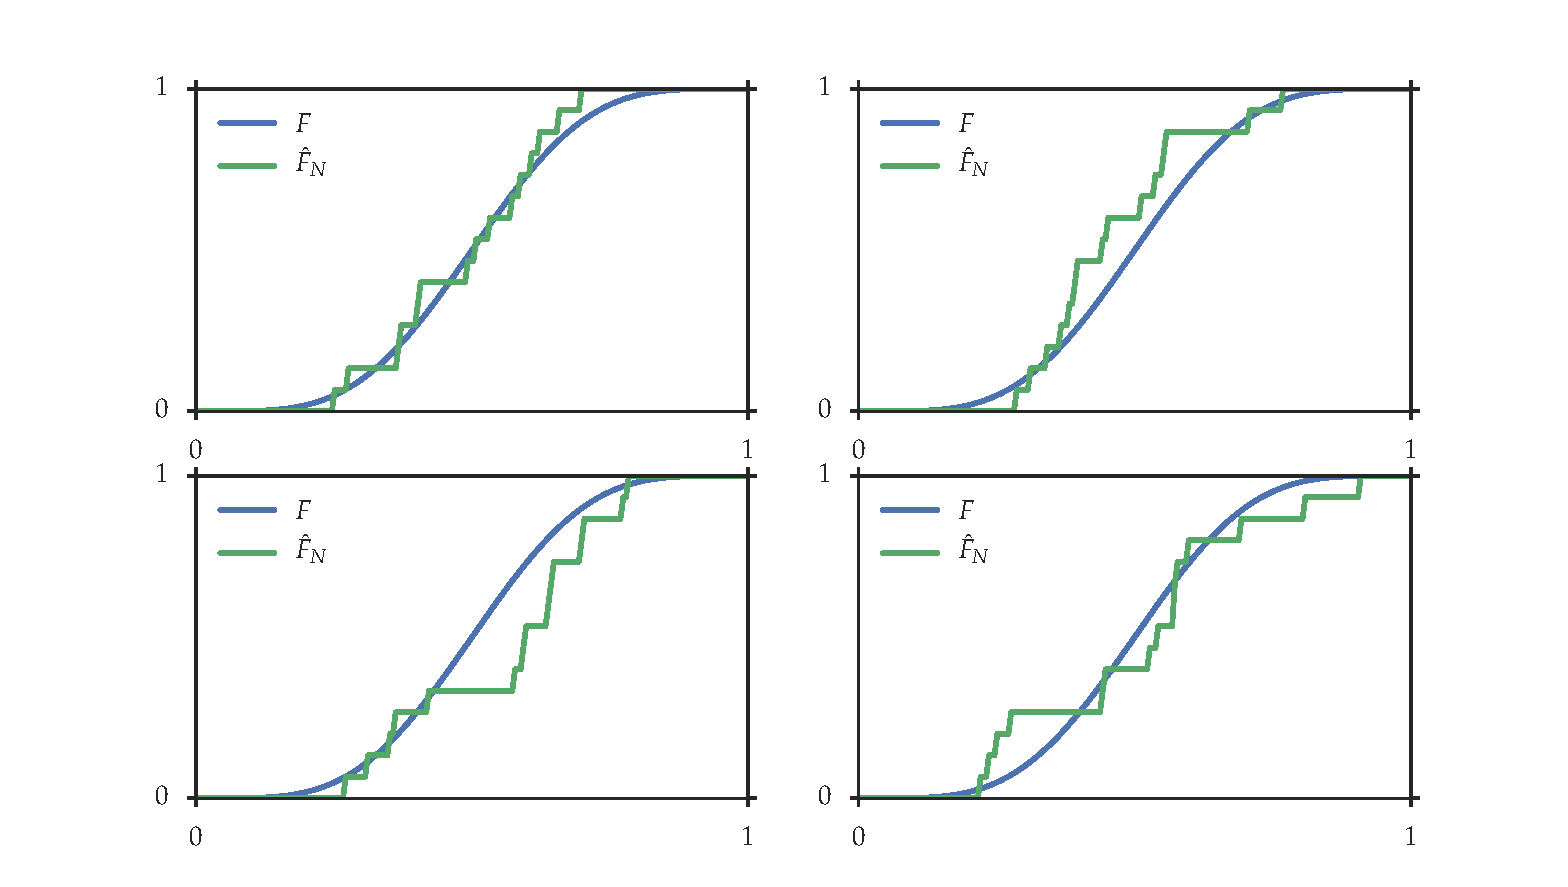
\includegraphics[trim={4em 4em 4em 2em}, clip]{ecdf_beta.pdf}}
    \caption{\label{f:ecdf_beta} $F$ and four observations of $\hat F_N$ when $N=15$. 
                Draws from a Beta$(5,5)$ distribution }
   \end{center}
    \end{figure}
    
\end{frame}

\begin{frame}\frametitle{Convergence}

    \vspace{2em}
    The empirical distribution is asymptotically an excellent estimator of $P$
    
    \vspace{.7em}
    If $\boldz_1, \ldots, \boldz_N$ are {\sc iid} 
    with common distribution $P$ and $\hat P_N$ is the empirical distribution,
    then, by the law of large numbers,
    %
    \begin{equation*}
        \hat P_N(B) = \frac{1}{N} \sum_{n=1}^N \1\{\boldz_n \in B\}
        \toprob 
        \PP\{\boldz_n \in B\} = P(B)
    \end{equation*}
    %
    for any Borel set $B$
    
\end{frame}

\begin{frame}
    
    \vspace{2em}
    Specializing to the scalar case with $B := (-\infty, s]$, we 
    have $\hat F_N(s) \toprob F(s)$ for any $s \in
    \RR$, where $F$ is the {\sc cdf} of $P$
    
    \vspace{.7em}
    Stronger result:
    
    \Thm \eqref{ET-t:fts}(\navy{Glivenko--Cantelli})
    Let $x_1, \ldots, x_N$ be {\sc iid} draws from $F$.  If $\hat F_N$ is the
    corresponding {\sc ecdf},  then
    %
    \begin{equation*}
        \label{eq:dev}
        \| F - \hat F_N \|_{\infty}
        \toprob 0
        \quad \text{as} \quad
        N \to \infty
    \end{equation*}
    %
    a.k.a. fundamental theorem of statistics 
    
\end{frame}

\begin{frame}

    \vspace{2em}
    The supremum norm:
    %
    \begin{equation*}
        \| F - \hat F_N \|_{\infty}
        := \sup_{s \in \RR} |\hat F_N(s) - F(s)| 
    \end{equation*}
    %
    Roughly, the maximal deviation over the domain
    
    \vspace{2em}
    In fact the
    convergence occurs ``almost surely,'' which is a stronger notion than in
    probability
    
\end{frame}

\begin{frame}

    \begin{figure}
   \begin{center}
    \scalebox{.42}{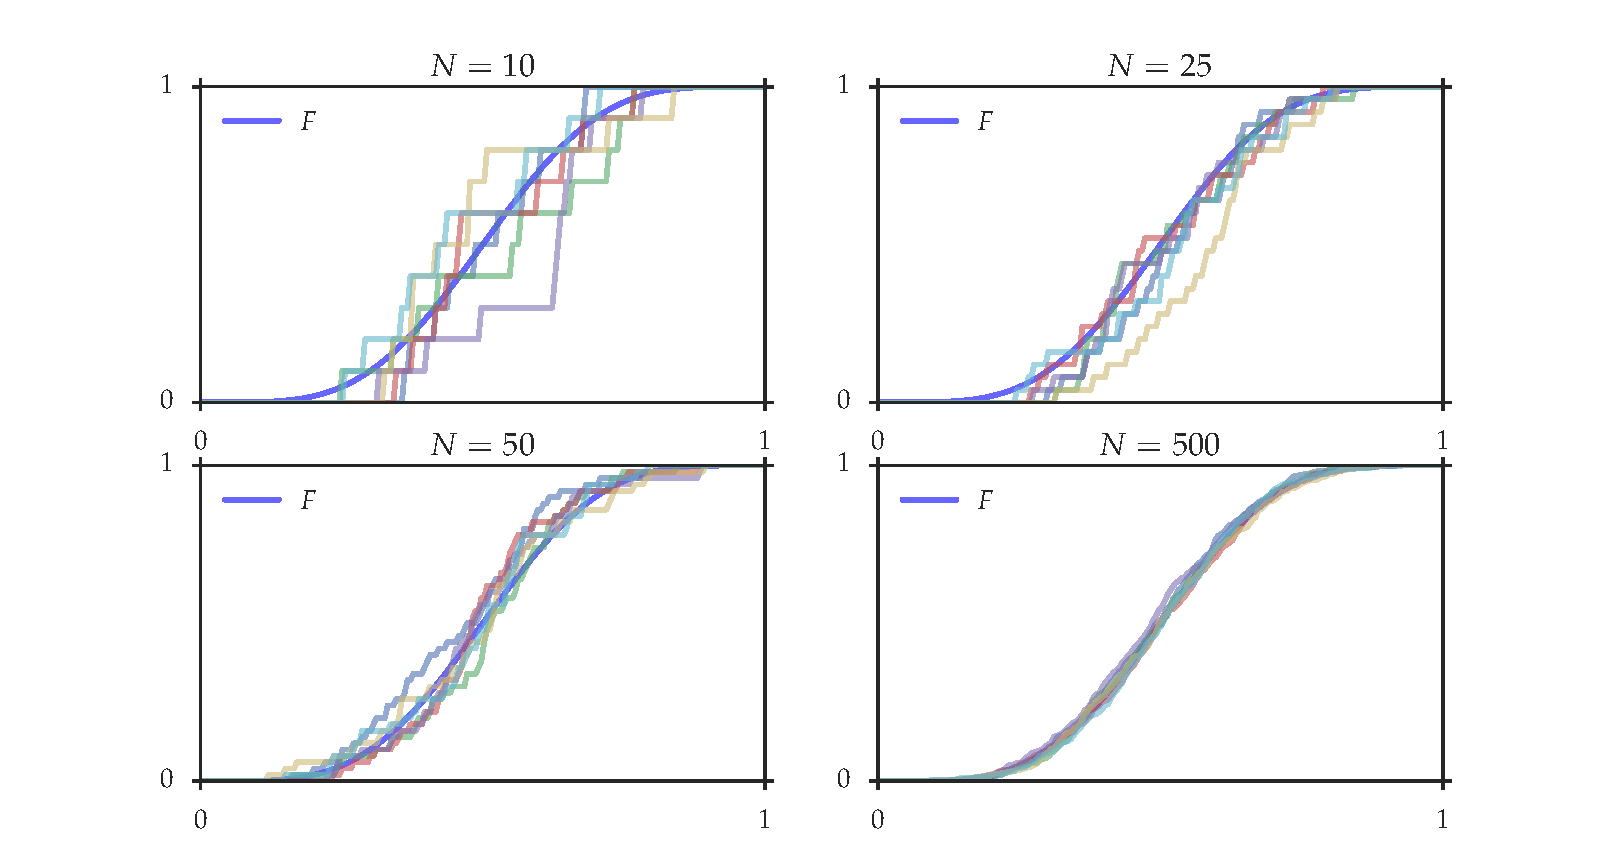
\includegraphics[trim={2em 3em 3em 1em}, clip]{ecdf_lim.pdf}}
    \caption{\label{f:ecdf_lim} Realizations of $\hat F_N$ with four different
    sample sizes. Independent draws from Beta(5,5)}
   \end{center}
    \end{figure}
    
\end{frame}

\begin{frame}

    \vspace{2em}
    Theorem~\ref{ET-t:fts}: in the {\sc iid} setting, with infinite amount 
    of data, we can learn the underlying distribution without any assumptions
    
    \vspace{.7em}
    Once
    we know the distribution $P$, we know any feature $\gamma = \gamma(P)$
    
\end{frame}

\begin{frame}
    
    \vspace{2em}
    Does knowing we can learn the underlying distribution in the limit offer
    any solution to the problem of estimation? No:

    \begin{itemize}
        \item in practice, we only
    ever have a finite amount of data
        \item the estimation problem was about inference -- there's no
                need to generalize if we know the full population
        \item with finite amount of data, empirical
        distribution treats
        the sample like the unknown distribution-- extreme form of
        over-fitting
    \end{itemize}
    
\end{frame}


\begin{frame}\frametitle{Identification}
    A class of distributions $\pP = \{P_{\boldtheta}\}$ indexed by $\boldtheta \in
    \Theta$ is called \navy{identifiable} if the map $\boldtheta \mapsto
    P_{\boldtheta}$ is one-to-one
    on $\Theta$

\end{frame}

\begin{frame}

    \vspace{2em}
    \Eg
    Recall the set of 
    all univariate normal distributions with positive variance:
    %
    \begin{align*}
        \pP := 
        \bigg\{
        \text{all } p \; \st \;
        p(s) = \frac{1}{\sqrt{2 \pi} \sigma}
       \exp \left\{ - \frac{(s - \mu)^2}{2\sigma^2} \right\}
       \; \\ \text{ for some }
       \; \mu \in \RR, \; \sigma > 0
       \bigg\}
    \end{align*}
    %
    This class is identifiable.
    
    \vspace{.7em}
    We can show that if $(\mu_a, \sigma_a)$ and $(\mu_b,
    \sigma_b)$ are distinct vectors, then the distributions $\nN(\mu_a,
    \sigma^2_a)$ and $\nN(\mu_b, \sigma^2_b)$ differ at at least one point
    
\end{frame}

\begin{frame}
    
    \vspace{2em}
    Identifiability means the parameter vector associated with
    the unknown distribution can eventually be distinguished from the data:
    
    \begin{itemize}
        \item suppose $\{P_{\boldtheta}\}$ is identified on $\Theta$ and
            nature generates an infinite sequence of observations $\{\boldz_n\}$ from $P = P_{\boldtheta}$
        \item let $\boldtheta'$ be any other vector in $\Theta$ and let
    $P'= P_{\boldtheta'}$
        \item  by identifiability, there exists at least one Borel set
    $B$ with $P(B) \not= P'(B)$
        \item since the empirical distribution $\hat P_N(B)$
        converges to $P(B)$, we can in the limit conclude that the data are not
        generated by $P'$
    \end{itemize}
    
\end{frame}

\section{Estimation Principles}

\begin{frame}\frametitle{The Sample Analogue Principle}

    \vspace{2em}
    Most of the estimators defined above can be derived from the \navy{plug-in method}, 
        also reffered to as ``analogue estimation" or \navy{sample analogue principle}: 
    %
    \begin{equation*}
        \text{to estimate } \gamma(P),\;
        \text{ use } \,
        \gamma(\hat P_N)
    \end{equation*}
    
    $\hat P_N$ is the empirical distribution constructed from the sample
    
    \vspace{2em}
    We replace the unknown distribution 
    $P$ with the observable distribution $\hat P_N$ and then 
    evaluate $\gamma(\hat P_N)$
\end{frame}

\begin{frame}
    
    \vspace{2em}
    \Eg
    Let $x_1, \ldots, x_N$ be draws from unknown distribution $P$.
    Suppose we want to estimate the mean $\gamma(P) := \int sP(\diff s)$.
    The sample analogue principle  tells us to replace $P$ with  
    $\hat P_N$, which gives
    %
    \begin{equation*}
        \gamma(\hat P_N) = \int s \hat P_N(\diff s) = \bar x_N
    \end{equation*}
    %
    
    Thus the sample mean is the estimator of the mean produced by the sample
    analogue principle
    
\end{frame}

\begin{frame}

    \vspace{2em}
    The $k$th sample moment applies the same principle to estimate the $k$th moment
    
    \vspace{.7em}
    \Eg
    When it exists, the variance of $P$ can be written as 
    %
    \begin{equation*}
        \sigma^2 = \gamma(P) = \int \left[ t - \int s P(\diff s) \right]^2
        P(\diff t)
    \end{equation*}
    %
    Applying the sample analogue principle leads to the estimator
    %
    \begin{equation*}
        \int \left[ t - \int s \hat P_N(\diff s) \right]^2 \hat P_N(\diff t)
            = \frac{1}{N} \sum_{n=1}^N (x_n - \bar x_N)^2
    \end{equation*}
    %
    This is precisely the sample variance

\end{frame}

\begin{frame}
    
    \vspace{2em}
    Other estimation methods that can be obtained as special
    cases of the sample analogue principle include:
    \begin{itemize}
        \item least squares regression
        \item maximum likelihood
        \item the method of moments
        \item generalized method of moments
    \end{itemize}
    
\end{frame}

\begin{frame}\frametitle{Best Linear Prediction}
    
    \vspace{2em}
    Recall the best linear prediction problem: $\alpha$
    and $\beta$ are chosen to minimize $\EE[ (y - \alpha - \beta x)^2 ]$
    
    \vspace{.7em}
    Letting $P$ be the distribution of $(x, y)$:
    %
    \begin{equation*}
        \label{eq:lstmp}
        (\alpha^*, \beta^*)
        = \gamma(P) := \argmin_{\alpha, \beta \in \RR} \int [ (t - \alpha - \beta
        s)^2 ] P(\diff s, \diff t)
    \end{equation*}
    
\end{frame}

\begin{frame}

    \vspace{2em}
    Corresponding statistical problem: produce the best linear predictor based
    only on a sample $\zdata = ((x_1, y_1), \ldots, (x_N, y_N))$ of observations
    from $P$
    
    \vspace{.7em}
    Given $\zdata$, form the empirical
    distribution:
    %
    \begin{equation*}
        \hat P_N(B) = \frac{1}{N} \sum_{n=1}^N \1\{(x_n, y_n) \in B\}
    \end{equation*}
    %
    This is the simple linear bivariate least squares problem.  The minimizers are 
    %
    \begin{equation*}
        \label{eq:solse}
        \hat \beta_N = \frac{\sum_{n=1}^N (x_n - \bar x_N)(y_n - \bar y_N)}
                        {\sum_{n=1}^N (x_n - \bar x_N)^2}
        \quad \text{and} \quad
        \hat \alpha_N = \bar y_N 
            - \hat \beta_N \bar x_N
    \end{equation*}
    
\end{frame}

\begin{frame}\frametitle{Limitations} 

    \vspace{1em}
    Sample analogue principle can fail. For example:
    
    \begin{itemize}
        \item let $\pP$ be the set of absolutely continuous distributions on $\RR$
        \item data generated by $P$ with 
        density
        %
        \begin{equation}
            \label{eq:denasf}
            \gamma(P) = DP
        \end{equation}
        %
        where $DP :=$ the derivative of the {\sc cdf} $F$ of $P$
        
        \item let $\hat P_N$ be the empirical distribution from a sample
    \end{itemize}
    
    Plug empirical distribution into the right-hand side
    of \eqref{eq:denasf}: since $\hat F_N$ is a step function,
    the derivative is zero everywhere, except at a finite number
    of jump points where the derivative is undefined 
        
\end{frame}

\begin{frame}\frametitle{Regularization}

    \vspace{2em}
    One interpretation of limitation: we need to combine the data with
    some kind of \navy{regularization}
    
    \vspace{.7em}
    Regularization:
    \begin{itemize}
        \item  penalize
            complexity or impose some kind of ``smoothing" a
            priori
        \item not
    grant the empirical distribution equal status with the unknown true
    distribution
        \item  regard the empirical distribution 
    only as partial information, and seek to 
    combine it with some form of prior information or external theory
    
    \end{itemize}
  
\end{frame}

\section{Empirical Risk Minimisastion}

\begin{frame}\frametitle{Empirical Risk Minimisation}

    \vspace{2em}
    Empirical risk minimization,  or ERM: the terminology and main
    concepts come from the machine learning literature
    
    \vspace{.7em}
    Nonetheless, many
    standard estimators in econometrics are special cases of ERM, including
    maximum likelihood and least squares
    
\end{frame}

\begin{frame}

    \vspace{2em}
    We observe an input $\boldx \in \RR^K$ to
    a system, followed by a scalar output $y$
    
    Both are random variables
    and the joint distribution of $\boldz := (\boldx, y)$ is $P$
    
    Our aim is to predict new output values from observed input values
    
    We'll do this
    by choosing a function $f$ such that $f(\boldx)$ is our prediction of $y$ once
    $\boldx$ is observed
    
    \vspace{.7em}
    In the machine learning literature, $f$ is called a
    \navy{prediction rule}
    
    In economics, $f$ is called a \navy{strategy} or
    \navy{policy function}
    
\end{frame}

\begin{frame}

    \vspace{2em}
    Incorrect prediction incurs a loss $L(y,
    f(\boldx))$
    
    \vspace{.7em}
    The function $L$  called the \navy{loss function}

    Common
    choices:
    
    \begin{itemize}
        \item the \navy{quadratic loss function} $L(y, f(\boldx)) = (y -
            f(\boldx))^2$
        \item the \navy{absolute deviation loss function} $L(y, f(\boldx)) = |y -
            f(\boldx)|$
        \item the \navy{discrete loss function} $L(y, f(\boldx)) = \1\{y \not=
            f(\boldx)\}$
    \end{itemize}

\end{frame}

\begin{frame}

    \vspace{2em}
    Given loss function $L$, choose $f$ to minimize the
    \navy{prediction risk} or prediction error, defined as the expected loss
    %
    \begin{equation*}
        \label{eq:rf}
        R(f) := \EE L(y, f(\boldx)) 
    \end{equation*}
    
    
    Expectation computed using the joint distribution $P$ of $(\boldx, y)$
    
    
\end{frame}

\begin{frame}

    \vspace{2em}
    \Eg
        Let $L$ be the quadratic loss function
        
        As shown in \S\ref{ET-ss:ce},
        the minimizer of $R(f)$ is the regression function, defined 
        at $\boldx$ by $f^*(\boldx) = \EE[y \given \boldx]$
        
        For any alternative policy $g$
        we have
        %
        \begin{equation}
            \label{eq:ebrf2}
            R(g) =  R(f^*) + \EE[ (f^*(\boldx) - g(\boldx))^2 ] 
        \end{equation}
        %
        With quadratic loss, good prediction equates to choosing
        $g$ to be close to the regression function,  minimizing the second
        term on the right-hand side of \eqref{eq:ebrf2}
        
        The term $R(f^*)$ represents a lower bound for
        prediction risk
        
\end{frame}

\begin{frame}

    \vspace{2em}
    In a statistical setting, we cannot evaluate $\EEP$
    
    We do have access to data
    $\boldz_1, \ldots, \boldz_N$, where each pair $\boldz_n = (\boldx_n, y_n)$ is
    an independent draw from $P$
    
    \vspace{.7em}
    Apply the
    sample analogue principle, replace $P$ in the risk function with $\hat P_N$:
    %
    \begin{equation*}
        \label{eq:erf}
        \Remp(f) 
        := \mathbb{E}_{\hat P_N} L(y, f(\boldx))
        = \frac{1}{N} \sum_{n=1}^N L(y_n, f(\boldx_n))
    \end{equation*}
    %
    .....this is called empirical risk
    
\end{frame}

\begin{frame}

    The problem to solve:
    %
    \begin{equation}
        \label{eq:minempr}
        \hat f = \argmin_{f \in \hH} \Remp(f)
    \end{equation}
    %
    Restrict domain to a class of functions $\hH$ called the \navy{hypothesis space}
    
\end{frame}

\begin{frame}
    
    \vspace{2em}
    Should we set $\hH$ to be the set of all
    functions $f \colon \RR^K \to \RR$?
    
    If the risk-minimizing
    function $f^* := \argmin_f R(f)$ is not in $\hH$, 
    then the solution to \eqref{eq:minempr} is not equal
    to $f^*$ and we are making a suboptimal choice
    
    \vspace{.7em}
    More soon, but this reasoning false:
    \begin{itemize}
        \item  we are solving a complex problem on the basis of
    limited information
        \item better to be restrictive in choice of hypothesis space
        \item key point: minimising empirical risk not the same
        as minimising prediction risk
    \end{itemize}
    
\end{frame}

\begin{frame}

    \begin{figure}
       \begin{center}
            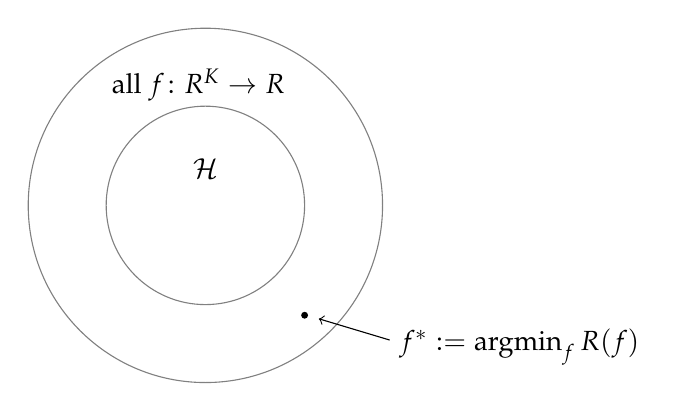
\begin{tikzpicture}[scale=0.9]
                \draw[gray] (0,0) circle (1.4cm);
                \node at (0,0.8) [below] {$\hH$};
                \draw[gray] (0,0) circle (2.5cm);
                \node at (-0.1,1.7) {all $f \colon \RR^K \to \RR$};
    
              \draw[fill=black] (1.4,-1.55) circle (0.04cm);
              \draw[<-] (1.6,-1.6) -- (2.6,-1.9);
              \node at (2.6,-2) [right] {$f^* := \argmin_f R(f) $};
            \end{tikzpicture}
            \caption{\label{f:circles} Choosing the hypothesis space}
       \end{center}
    \end{figure}
    
\end{frame}


\begin{frame}

    \vspace{2em}
    \Eg
    Specializing ERM problem to scalar $x$ and quadratic 
    loss function $L(y, f(x)) = (y - f(x))^2$:
    %
    \begin{equation*}
        \label{eq:ermlsq}
        \min_{f \in \hH} \; \sum_{n=1}^N (y_n - f(x_n))^2
    \end{equation*}
    %
    This is the \navy{least
    squares problem}
    
    \vspace{.7em}
    We can specialize $\hH$ to be the set of affine functions
    %
    \begin{equation}
        \label{eq:allaff}
        \llL := \{ \text{ all functions of the form } \ell(x) = \alpha + \beta x \}
    \end{equation}
    
\end{frame}

\begin{frame}

    \vspace{2em}
    Problem becomes the \navy{simple linear least squares problem} 
    %
    \begin{equation}
        \label{eq:llsp}
        \min_{\ell \in \, \llL} \; \sum_{n=1}^N (y_n - \ell(x_n))^2
        = \min_{\alpha, \, \beta } \, \sum_{n=1}^N  (y_n - \alpha - \beta x_n)^2  
    \end{equation}
    
\end{frame}

\begin{frame}
    
    \vspace{2em}
    Two approaches, same solution
    
    Sample analouge principle
    \begin{itemize}
        \item plug in empirical distribution and solve the best 
            linear preduction problem 
    \end{itemize}
    
    \vspace{.7em}
    Empirical risk minimisation 
    \begin{itemize}
        \item trying to find
            the best predictor
        \item at the same time, we restrict ourselves to linear
            approximations in recognition of the
            limited information we are basing our prediction on 
    \end{itemize}
    
\end{frame}

\begin{frame}{Quantile Regression}

    \vspace{2em}
    Quantile regression: estimate a quantile of a given distribution based on a set of
    predictive variables
    
    \vspace{.7em}
    For example, quantile regression to
    estimate quantiles of CEO compensation as function of the
    market value of their firms (\citeauthor{koenker2001quantile} \citeyear{koenker2001quantile})
    
    \vspace{.7em}
    Quantile regression can be regarded as a special
    case of empirical risk minimization
    
\end{frame}

\begin{frame}
    
    \vspace{2em}
    Let $F$ be a strictly increasing {\sc cdf} on $\RR$ and let $\tau \in (0, 1)$ be given
    
    Recall from \S\ref{ET-ss:quantile} in ET that the $\tau$th quantile of $F$
    is the $\xi$ that solves $F(\xi) = \tau$
    
    \vspace{.7em}
    We can define the $\tau$th quantile as the
    solution to:
    %
    \begin{equation*}
        \label{eq:altxi}
        \min_{\xi \in \RR} \, \EE L_\tau (y, \xi) 
    \end{equation*}
    %
    where $y$ is a random variable with distribution $F$ and
    %
    \begin{equation*}
        L_\tau (y, \xi)
        := | (y - \xi) (\tau - \1\{y < \xi\}) | 
    \end{equation*}
    %
    (See exercise~\ref{ET-ex:quantreg} in ET)
    
\end{frame}

\begin{frame}
    
    \vspace{2em}
    We now want to estimate the $\tau$th quantile of $F$ using some
    input variable $x$ (e.g., a CEO compensation quantile as a function
    of firm size)
    
    \vspace{.7em}
    Frame the
    search for a suitable function as a problem of minimizing the prediction 
    %
    \begin{equation*}
        \label{eq:altxi2}
        R(f) := \, \EE L_\tau (y, f(x))
    \end{equation*}
    %
    Use the principle of empirical
    risk minimization with data set $(x_1, y_1), \ldots, (x_N, y_N)$
    
    We get $\min_{f \in \hH} \; \sum_{n=1}^N L_\tau (y_n , f(x_n))$,
    where $\hH$ as the hypothesis space
    
    
    
\end{frame}

\begin{frame}

    \vspace{2em}
    When $\hH = \llL$, the set of affine functions, the ERM problem
    is
    %
    \begin{equation*}
        \min_{\alpha, \, \beta } \, \sum_{n=1}^N 
        | (y_n - \alpha - \beta x_n) (\tau - \1\{y_n < \alpha + \beta x_n\}) | 
    \end{equation*}
    %
    Standard expression for the quantile regression problem
    
    \vspace{.7em}
    If $\tau = 0.5$, then the objective function is proportional to $\sum_{n=1}^N | y_n -
    \alpha - \beta x_n |$ ---  called \navy{median regression} or \navy{least
    absolute deviation regression} 

    
\end{frame}

\begin{frame}\frametitle{The Choice of Hypothesis Space}
    
    \vspace{2em}
    \Fact\eqref{ET-fa:emprd}
        Let $\hH_1$ and $\hH_2$ be two hypothesis spaces.
        If $\hat f_i$ is the empirical risk minimizer over $\hH_i$ as defined in
        \eqref{eq:minempr}, then 
        %
        \begin{equation*}
        \hH_1 \subset \hH_2 \implies \Remp(\hat f_1) \geq \Remp(\hat f_2)
        \end{equation*}
        %
    
    \vspace{.7em}
    
    We can always decrease empirical risk by increasing the
    hypothesis space

    
\end{frame}

\begin{frame}\frametitle{Empirical Versus Prediction Risk}
    
    \vspace{2em}
    Prediction risk of predictor $f$ measures the \navy{out-of-sample fit} of $f$:
    
    \begin{itemize}
        \item expected performance of $f$ when confronted with new data
        \item statistical procedure that produces a
                predictor $f$ with low prediction risk means that we have succeeded
                in meeting the goal of \emph{generalizing} from data
        \item  prediction risk unobservable
    \end{itemize}
    
    \vspace{.7em}
    Empirical
    risk measures \navy{in-sample fit} of $f$:
    \begin{itemize}
    \item empirical
    risk is a downward biased
    estimator of risk
    \item as we vary the hypothesis space, 
    prediction risk can rise even when empirical risk is falling
    \end{itemize}
    
\end{frame}

\begin{frame}
    
    \vspace{2em}
    We consider example where empirical risk is minimized
    over progressively larger hypothesis spaces
    
    \vspace{.7em}
    Generate input-output pairs via
    %
    \begin{equation*}
        x \sim U[-1,1] \;\; \text{ and then } \;\; y = \cos(\pi x) + u
        \;\; \text{ where }\;\;  u \sim N(0,1)
    \end{equation*}
    
    $U[-1,1]$ is the uniform distribution on the interval $[-1,1]$
    
\end{frame}


\begin{frame}

    \vspace{2em}
    Hypothesis spaces for predicting $y$ from $x$ will be sets of polynomial
    functions
    
    \vspace{.7em}
    Let $\pP_d$ be the set of all polynomials of
    degree $d$:
    %
    \begin{align*}
        \pP_d := \{ \text{ all functions } f_d(x) = c_0 x^0 + c_1 x^1 + \cdots c_d
        x^d \\ \text{ where each } c_i \in \RR \}
    \end{align*}
    
    Sequence of hypothesis spaces is increasing:
    %
    \begin{equation*}
        \pP_1 \subset \pP_2 \subset \pP_3 \subset \cdots
    \end{equation*}
    
\end{frame}

\begin{frame}
    
    \vspace{2em}
    Using quadratic loss and the
    set $\pP_d$ as our candidate functions, the risk minimization problem is
    %
    \begin{equation*}
        \label{eq:rminpoly}
        \min_{f \in \pP_d} R(f) 
        \quad \text{where} \quad 
        R(f) = \EE[ (y - f(x))^2 ]
    \end{equation*}
    %
    
    The empirical risk minimization problem: 
    %
    \begin{equation}
        \label{eq:erminpoly}
        \min_{f \in \pP_d} \Remp(f) 
        \quad \text{where} \quad 
        \Remp(f) = \frac{1}{N} \sum_{n=1}^N (y_n - f(x_n))^2
    \end{equation}
\end{frame}

\begin{frame}

    \vspace{2em}
    Experiment to demonstrate over-fitting: 
    \begin{enumerate}
        \item generate
    $N=25$ data points from the model -- data plotted as circles
        \item taking generated data, solve (\ref{eq:erminpoly}) repeatedly, 
        once for each $d$ in $1,2,\ldots,20$
        \item solution to the $d$th minimization problem is denoted $\hat f_d$ -- plotted in red
        \item compare the risk
    $R(\hat f_d)$ and empirical risk $\Remp(\hat f_d)$
    \end{enumerate}
    
\end{frame}

\begin{frame}

    \begin{figure}
   \begin{center}
    \scalebox{.4}{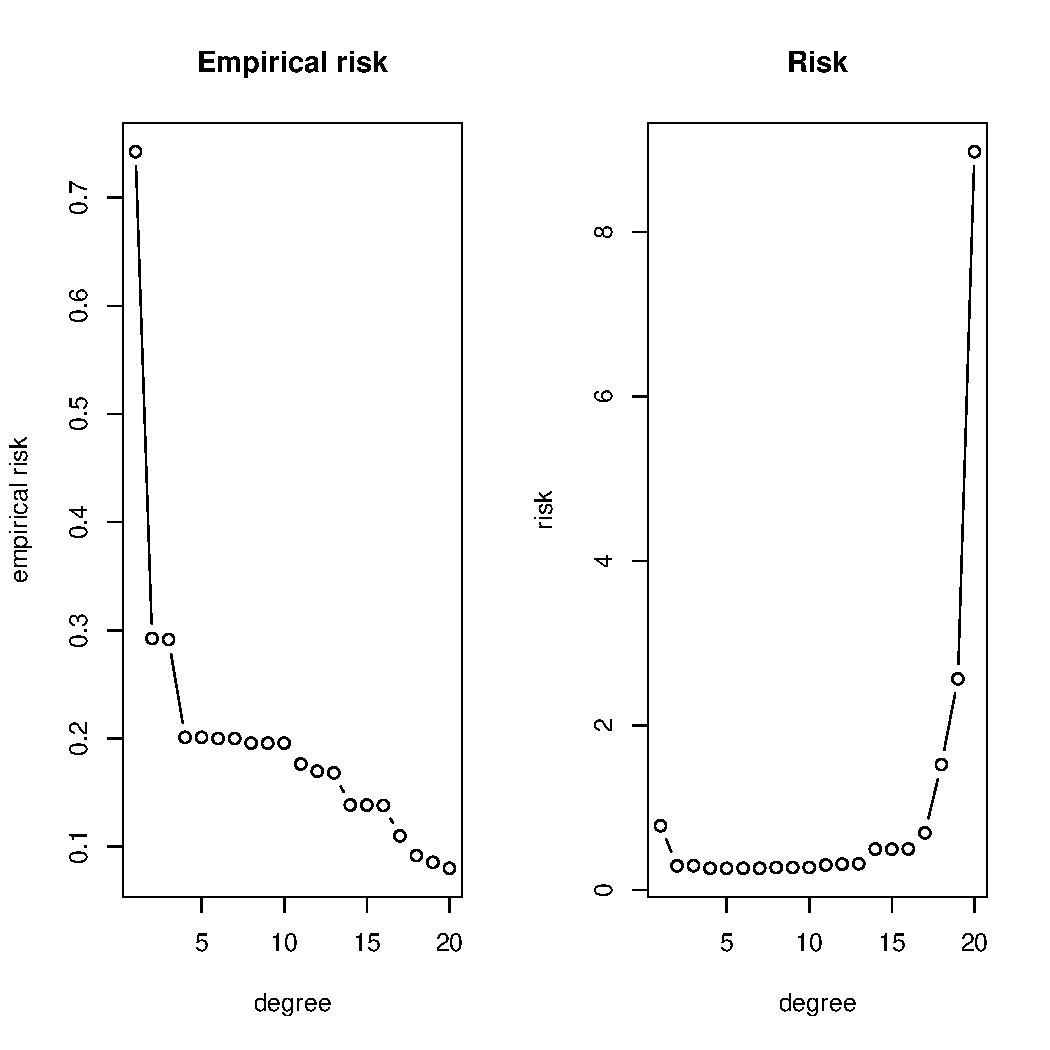
\includegraphics{rvempr.pdf}}
    \caption{\label{f:rvempr} Risk and empirical risk as a function of $d$}
   \end{center}
    \end{figure}
    
\end{frame}



\begin{frame}

    \begin{figure}
       \begin{center}
        \scalebox{.44}{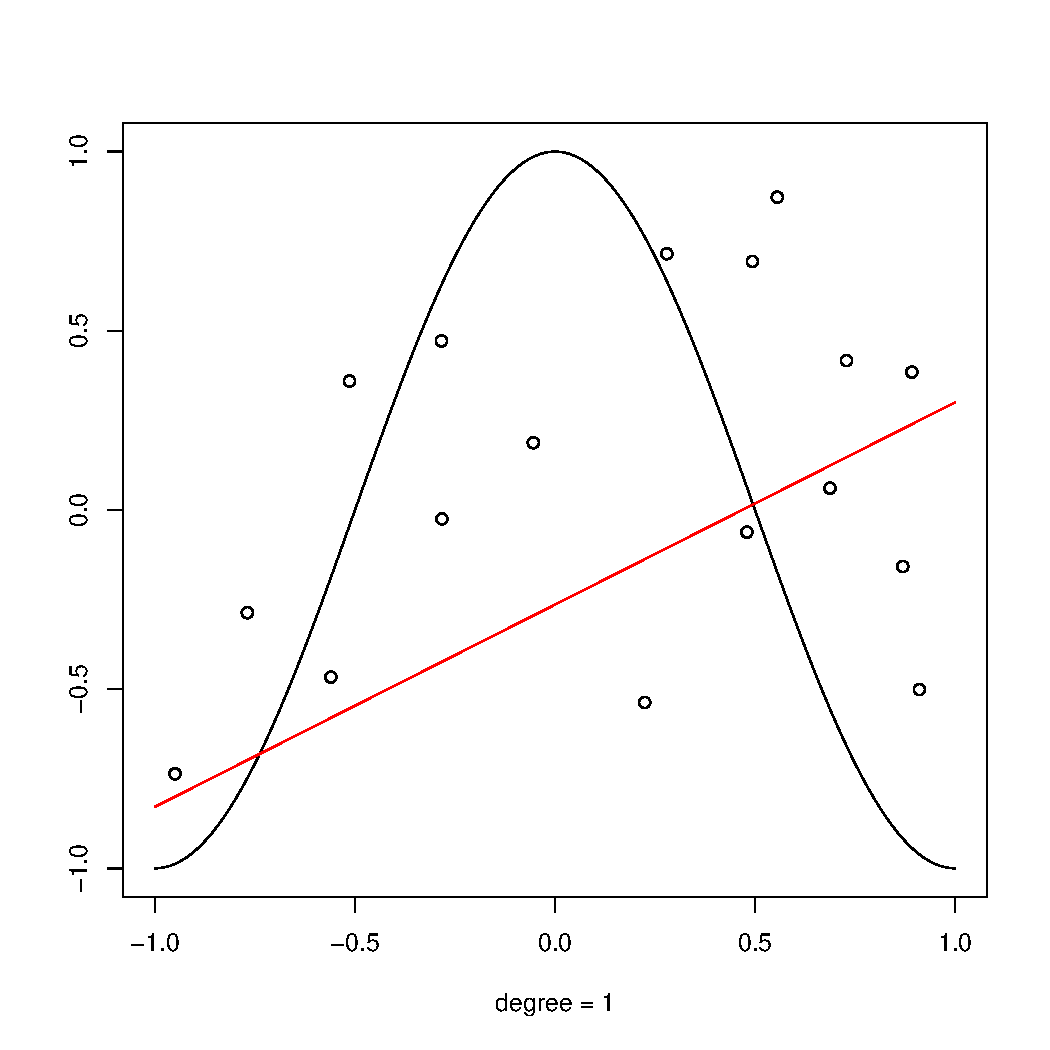
\includegraphics[trim={0em 0em 0em 2em}, clip]{ofit1.pdf}}
        \caption{\label{f:ofit1} Fitted polynomial, $d=1$}
       \end{center}
    \end{figure}
    
\end{frame}

\begin{frame}

    \begin{figure}
       \begin{center}
        \scalebox{.44}{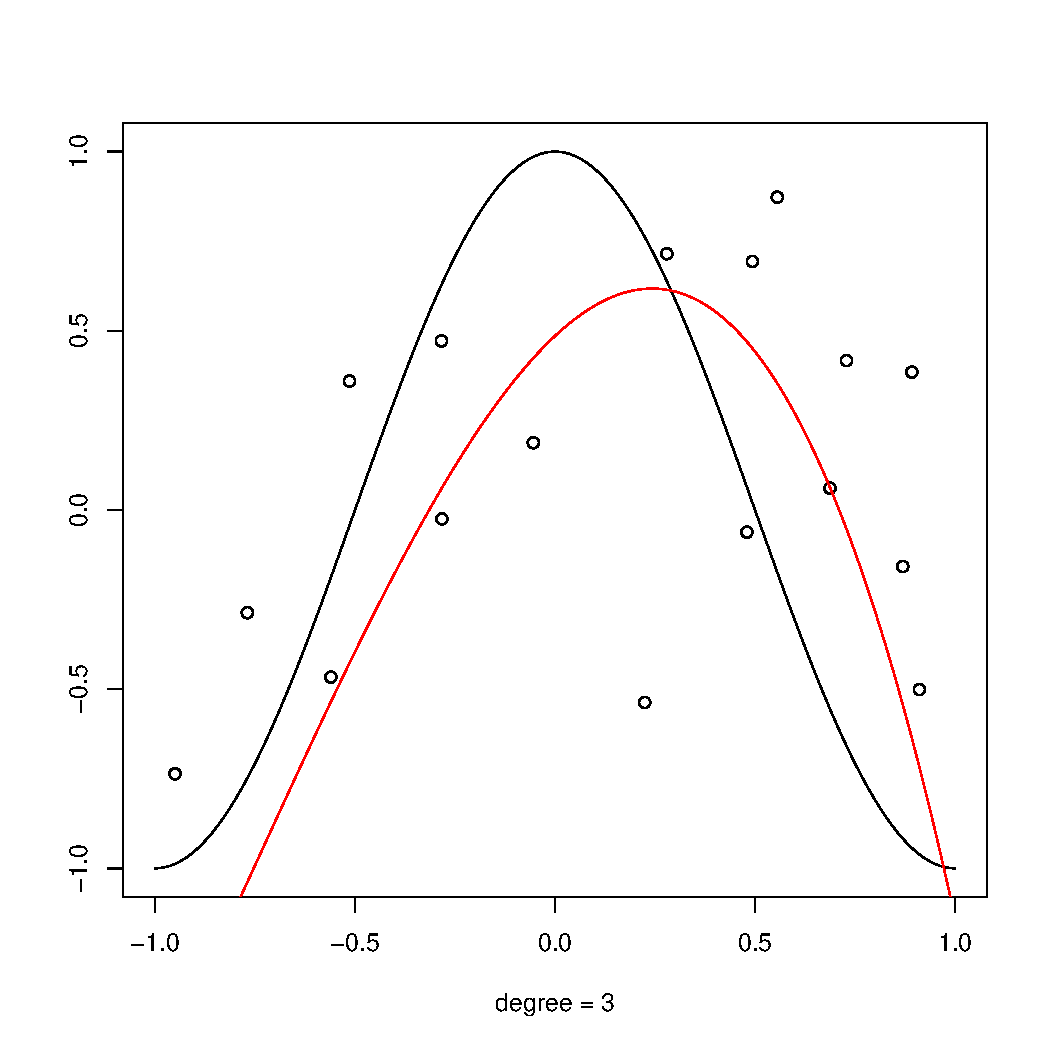
\includegraphics[trim={0em 0em 0em 2em}, clip]{ofit3.pdf}}
        \caption{\label{f:ofit3} Fitted polynomial, $d=3$}
       \end{center}
    \end{figure}
    
\end{frame}

\begin{frame}

    \begin{figure}
       \begin{center}
        \scalebox{.44}{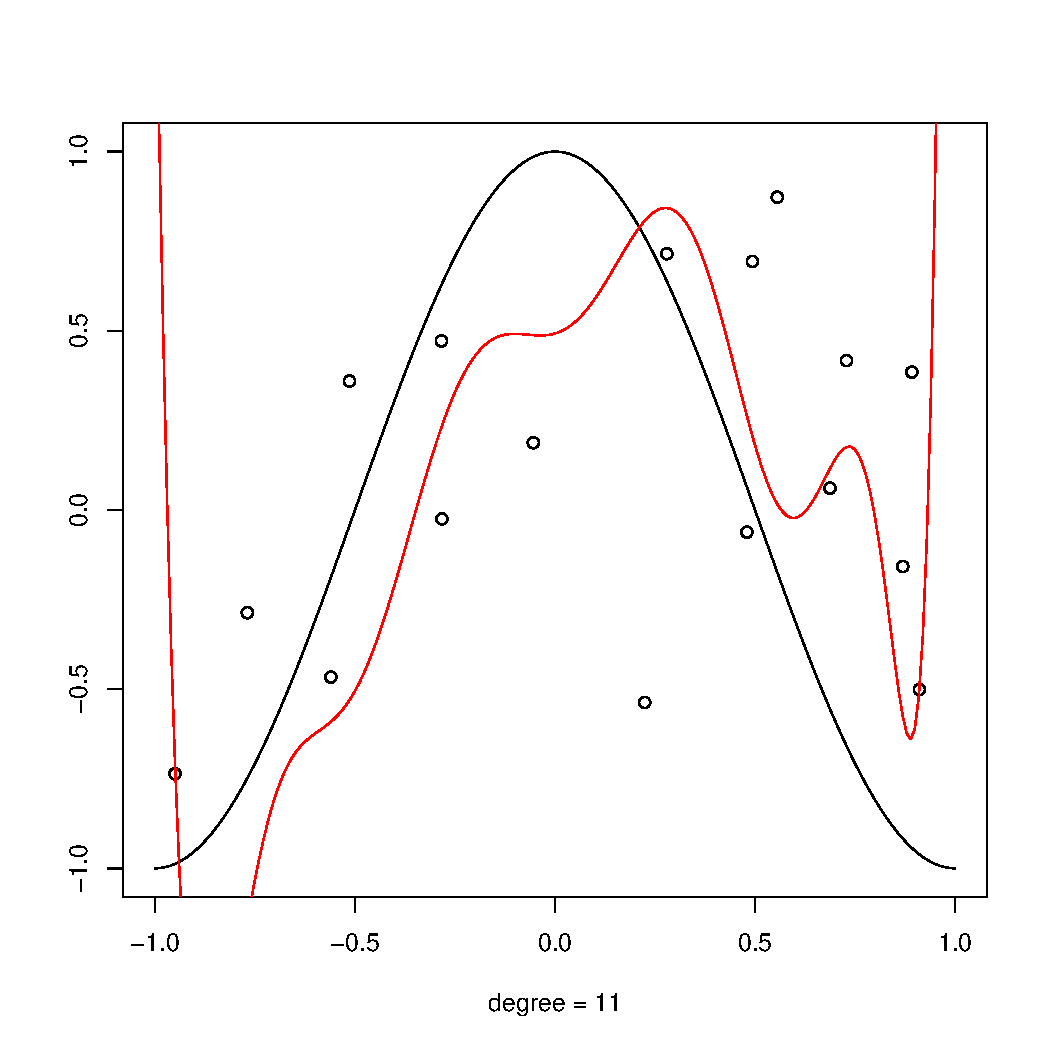
\includegraphics[trim={0em 0em 0em 2em}, clip]{ofit11.pdf}}
        \caption{\label{f:ofit11} Fitted polynomial, $d=11$}
       \end{center}
    \end{figure}
    
\end{frame}

\begin{frame}

    \begin{figure}
       \begin{center}
        \scalebox{.44}{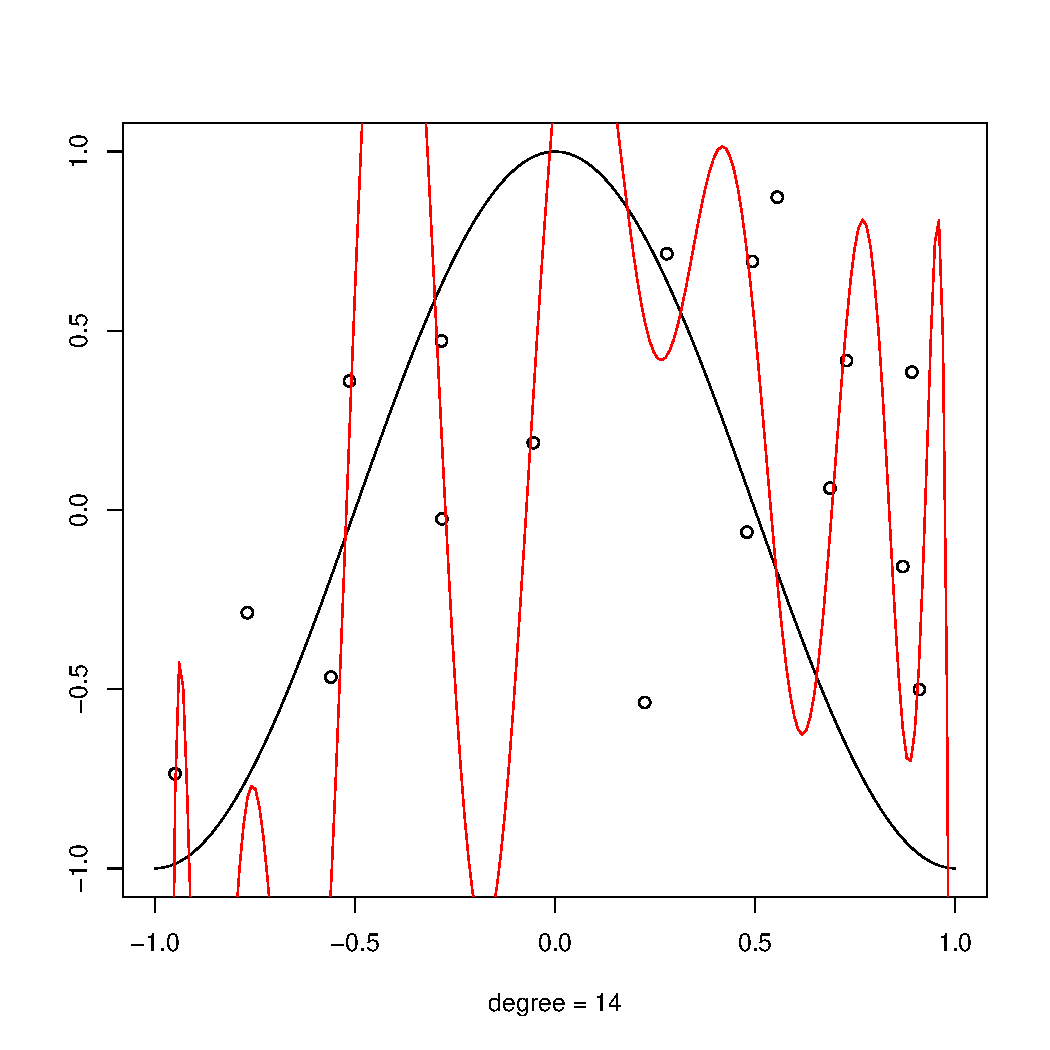
\includegraphics[trim={0em 0em 0em 2em}, clip]{ofit14.pdf}}
        \caption{\label{f:ofit14} Fitted polynomial, $d=14$}
       \end{center}
    \end{figure}
    
\end{frame}


\begin{frame}
    
    \vspace{2em}
    Empirical risk falls monotonically with $d$
    
    \vspace{.7em}
    But risk decreases slightly and then increases rapidly

    \begin{itemize}
        \item small $d$ (\navy{underfitting}): high empirical risk and high risk
        \item medium $d$: risk is minimized
        \item large $d$ (\navy{overfitting}): \underline{small empirical risk and high risk}
    \end{itemize}
    
    With large $d$, too much emphasis has been given to this particular
    realization of the data 

    High risk means large expected loss

\end{frame}

\begin{frame}

    In applications, we do not know the
    true data-generating process when we choose $\hH$
    \begin{itemize}
        \item best scenario: we have firm theory guiding us to 
        a suitable hypothesis space
        \item worst scenario: we have no idea and choose blindly
    \end{itemize}


\end{frame}

\section{Parametric Methods}

\begin{frame}\frametitle{Parametric Methods}
    Standard parametric estimation methods:
    \begin{itemize}
        \item maximum likelihood
        \item Bayesian estimation
        \item generalized method
    of moments
    \end{itemize}

\end{frame}

\begin{frame}{Maximum Likelihood}

    \vspace{2em}
    Suppose the data $x_1,\ldots,x_N$ has joint density $p$ 
    
    \vspace{.7em}
    Assume $p = p(\cdot \,; \boldtheta)$ is
    a member of a parametric class $\pP$ indexed by parameter vector $\boldtheta \in
    \Theta$
    
    \vspace{.7em}
    Each choice of $\boldtheta$ pins down a particular density $p =
    p(\cdot \,;
    \boldtheta)$, but $\boldtheta$ generating the data is unknown
    
\end{frame}

\begin{frame}

    \vspace{2em}
    The \navy{likelihood function} is $p$ evaluated at the sample
    $x_1,\ldots,x_N$
    
    \vspace{.7em}
    The likelihood function regarded as a function of $\boldtheta$:
    %
    \begin{equation*}
        \label{eq:deflf0}
        L(\boldtheta) := p(x_1,\ldots,x_N ; \boldtheta)
        \qquad (\boldtheta \in \Theta)
    \end{equation*}
    
\end{frame}

\begin{frame}

    \vspace{2em}
    The principle of maximum likelihood: estimate $\boldtheta$ by
    maximizing $L(\boldtheta)$ over $\boldtheta \in \Theta$
    
    A statistic $\hat \boldtheta$ is called a \navy{maximum likelihood estimate}
    (MLE) of $\boldtheta$ if 
    %
    \begin{equation*}
        \label{eq:defmle}
        \hat \boldtheta \in \argmax_{\boldtheta \in \Theta} L(\boldtheta) 
    \end{equation*}
    
    \vspace{.7em}
    Equivalent to maximizing the \navy{log likelihood function}
    %
    \begin{equation*}
        \ell(\boldtheta) := \ln (L(\boldtheta)) 
        \qquad (\boldtheta \in \Theta)
    \end{equation*}
    %
    The set of MLEs can be a singleton, contain multiple elements or be
    empty
    
\end{frame}

\begin{frame}

    \vspace{2em}
    If each $x_n$ is drawn independently from fixed arbitrary
    (marginal) density $p_n(\cdot \,; \boldtheta)$ on $\RR$, then
    %
    \begin{equation*}
        \label{eq:deflf}
        L(\boldtheta) = \prod_{n=1}^N p_n(x_n ; \boldtheta)
        \quad \text{and} \quad
        \ell(\boldtheta) = \sum_{n=1}^N \ln p_n(x_n ; \boldtheta)
    \end{equation*}
    %
    If each data point is multivariate, just replace $x_n$ with $\boldx_n$

    
\end{frame}

\begin{frame}

    \vspace{2em}
    \Eg
    Suppose that $x_1, \ldots, x_N$ are {\sc iid} draws from a normal
    distribution $\nN(\mu, v)$ with $\boldtheta = (\mu, v)$ unknown.
    The log likelihood function is
    %
    \begin{equation*}
        \ell(\mu, v) 
            = -\frac{N}{2} \ln (2 \pi v)
            - \frac{1}{2} \sum_{n=1}^N \frac{(x_n - \mu)^2}{v}
    \end{equation*}
    
    Joint maximization over $(\mu, v)$ gives the maximum likelihood estimators 
    %
    \begin{equation*}
        \label{eq:mlen}
        \hat \mu = \frac{1}{N} \sum_{n=1}^N x_n
        \quad \text{and} \quad
        \hat v = \frac{1}{N} \sum_{n=1}^N (x_n - \bar x_N)^2
    \end{equation*}
    
    \vspace{.7em}
    Thus, the MLEs of $\mu$ and $v$ are the sample mean and sample
    variance
    
\end{frame}

\begin{frame}

    \vspace{2em}
    MLE estimators typically have excellent asymptotic properties. However:
    
    \begin{itemize}
        \item attractive asymptotic theory dependent on correct specification 
        of the parametric class -- we must specify the entire joint distribution of the sample
        \item  good finite sample properties are not guaranteed
    \end{itemize}
    
\end{frame}

\begin{frame}\frametitle{Conditional Maximum Likelihood}

    \vspace{2em}
    Suppose we observe inputs $\boldx_1, \ldots,
    \boldx_N$ to some system and corresponding outputs $y_1, \ldots, y_N$
    
    \vspace{.7em}
    Assume $(\boldx_n, y_n)$ are {\sc iid}
    
    \vspace{.7em}
    Aim: estimate
    $\boldtheta$ in $p(y \given \boldx ; \boldtheta)$
    
    
\end{frame}

\begin{frame}

    \vspace{2em}
    We maximize 
    %
    \begin{equation*}
        \ell(\boldtheta) = \sum_{n=1}^N \ln p(\boldx_n, y_n; \boldtheta)
    \end{equation*}
    %
    $$\text{where} \quad
        p := \; \text{the joint density of } (\boldx_n, y_n)$$
    %
    
    \vspace{.7em}
    Letting $\pi$ be the marginal density of $\boldx$, we write 
    %
    \begin{equation*}
        p(\boldx, y; \boldtheta)
        = p( y \given \boldx; \boldtheta) \, \pi(\boldx)
    \end{equation*}
    %
    The density $\pi$ is unknown but we have not parameterized it because we
    aren't trying to estimate $\pi$
    
\end{frame}

\begin{frame}
    
    \vspace{2em}
    Rewrite the log likelihood as
    %
    \begin{equation*}
        \ell(\boldtheta) 
        = \sum_{n=1}^N \ln p(y_n \given \boldx_n; \boldtheta) 
        + \sum_{n=1}^N \ln \pi(\boldx_n) 
    \end{equation*}
    
    \vspace{.7em}
    Hence the MLE is
    %
    \begin{equation*}
         \argmax_{\boldtheta \in \Theta} \sum_{n=1}^N \ln p(y_n \given \boldx_n; \boldtheta)
    \end{equation*}
    %
    The objective function here is called
    the \navy{conditional log likelihood}
    
\end{frame}

\begin{frame}

    \vspace{2em}
    \Eg
    Consider a discrete response model with binary output $y_n$, where $y_n=1$
    indicates that the $n$th individual in a sample of women participates in
    the labor force
    
    This decision is influenced by a vector $\boldx_n$
    measuring characteristics such as income from the rest of the household
    
    \vspace{2em}
    Let 
    %
    \begin{equation*}
        q(\bolds) 
        := \PP\{ y = 1 \given \boldx = \bolds \}
        \qquad \left(\bolds \in \RR^K \right)
    \end{equation*}
    
    One modeling approach is to take $q(\bolds) = F(\boldbeta^\T \bolds)$,
    where $\boldbeta$ is a vector of parameters and $F$ is a specified {\sc cdf}
    
\end{frame}

\begin{frame}

    \vspace{2em}
    \Eg (cont.)
    We can then write
    %
    \begin{equation*}
        \PP\{ y = i \given \boldx = \bolds\} 
        = F(\boldbeta^\T \bolds)^i 
            (1 - F(\boldbeta^\T \bolds))^{1-i}
        \quad 
    \end{equation*}
    %
    $\text{for } \bolds \in \RR^K \text{ and } i \in \{0, 1\}$

    This is the conditional {\sc pmf} of $y$ given $\boldx$, so
    the conditional log likelihood of the sample is
    %
    \begin{align*}
        \ell(\boldbeta) 
        & = \sum_{n=1}^N \ln 
            [ F(\boldbeta^\T \boldx_n)^{y_n} (1 - F(\boldbeta^\T \boldx_n))^{1-y_n} ]
        \\
        & = \sum_{n=1}^N 
            y_n \ln F(\boldbeta^\T \boldx_n) + \sum_{n=1}^N (1 - y_n) \ln (1 -
            F(\boldbeta^\T \boldx_n))
    \end{align*}

\end{frame}

\begin{frame}

    \vspace{2em}
    \Eg (cont.)
    If $F$ is the standard normal {\sc cdf} $\Phi$, then this model is called
    the \navy{probit} model
    
    \vspace{.7em}
    If $F$ is the logistic {\sc cdf} $F(\bolds) =
    1/(1 + e^{-s})$, then it is called the \navy{logit} model

\end{frame}


\begin{frame}{Method of Moments and GMM}

     \vspace{2em}
    Estimate a vector $\boldtheta$ that solves an equation of the form
    %
    \begin{equation*}
        \label{eq:mm}
        g(\boldtheta) = \EE h( \boldx )
    \end{equation*}
    %
    The functions $g$ and $h$ are observable and vector-valued
    
    \vspace{.7em}
    We have observations $\boldx_1, \ldots, \boldx_N$ from $P$
    
    Apply sample analogue principle --- \navy{method of moments estimator} 
    is the solution $\hat \boldtheta$, if it
    exists, to the equation
    %
    \begin{equation}
        \label{eq:mme}
        g(\hat \boldtheta) = \frac{1}{N} \sum_{n=1}^N h(\boldx_n)
    \end{equation}

\end{frame}

\begin{frame}

    \vspace{2em}
    \Eg
    The mean of the Pareto distribution with scale parameter $s_0 = 1$ and
    shape parameter $\alpha$ is $\alpha /
    (\alpha - 1)$.  (If $\alpha > 1$.)
    
    \vspace{.7em}
    Letting $g(\alpha) := \alpha / (\alpha - 1)$:
    %
    \begin{equation*}
        g(\alpha) = \EE x
        \quad \text{where} \quad
        \lL(x) = \text{Pareto}(\alpha, 1)
    \end{equation*}
    
    \vspace{.7em}
    To estimate $\alpha$ with observations $x_1, \ldots, x_N$ from a
    $\text{Pareto}(\alpha, 1)$ distribution, solve $g(\hat \alpha) = \frac{1}{N}
    \sum_{n=1}^N x_n$ for $\hat \alpha$
    
    The result is
        $\hat \alpha := \bar x_N/(\bar x_N - 1)$

\end{frame}

\begin{frame}

    \vspace{2em}
    \navy{Generalized method of moments} (GMM) is a small step from method of moments
    
    If we express \eqref{eq:mm} above as $\EE[g(\boldtheta) - h(\boldx)] = \boldzero$, 
    then we can consider the more general expression
    %
    \begin{equation}
        \label{eq:gmm}
        \EE G(\boldtheta, \boldx) = \boldzero
    \end{equation}
    %
    This expression is called the \navy{orthogonality condition}
    
    \vspace{.7em}
    The generalized
    method of moments estimator of $\boldtheta$ is the solution $\hat \boldtheta$ to the
    empirical counterpart, which is
    %
    \begin{equation*}
        \label{eq:gmme}
        \frac{1}{N} \sum_{n=1}^N G(\hat \boldtheta, \boldx_n) = \boldzero
    \end{equation*}
    
\end{frame}

\begin{frame}

    \vspace{2em}
    Of course, no guarantee a solution will exist here
    \begin{itemize}
        \item the function $G$ can be nonlinear
        \item the number of
    equations can be greater than the number of unknowns --- \navy{overidentified} 
    \end{itemize}
    
    \vspace{.7em}
    When the system is overidentified, our study of overdetermined systems of
    equations in \S\ref{ET-ss:odse}
    suggests:
    %
    \begin{equation*}
        \label{eq:gmme2}
        \hat \boldtheta = \argmin_{\boldtheta \in \Theta} 
            \left \|
                \frac{1}{N} \sum_{n=1}^N G(\boldtheta, \boldx_n) 
            \right \|
    \end{equation*}
    
\end{frame}

\begin{frame}

    \vspace{2em}
    In practice, replace the
    Euclidean norm $\| \cdot \|$ with a weighted norm $\|
    \cdot \|_W$ defined by $\| \boldx \|_W^2 = \boldx^\T \boldW \boldx$,
    where $\boldW$ is a positive definite \navy{weighting matrix}
    \begin{itemize}
        \item  produce an estimator that has small variance asymptotically
    \end{itemize}

    \vspace{.7em}
    The estimation problem:
    %
    \begin{equation*}
        \label{eq:gmme3}
        \hat \boldtheta 
        = \argmin_{\boldtheta \in \Theta} 
        \left[ \frac{1}{N} \sum_{n=1}^N G(\boldtheta, \boldx_n) \right]^\T
        \hat \boldW
        \left[ \frac{1}{N} \sum_{n=1}^N G(\boldtheta, \boldx_n) \right]
    \end{equation*}
    %
    Note $\hat \boldW$ is allowed
    to depend on the sample

\end{frame}

\begin{frame}\frametitle{Bayesian Estimation}

    \vspace{2em}
    The main idea: treat parameters as unknown quantities
    for which we hold subjective beliefs regarding their values
    
    \vspace{.7em}
    These
    subjective beliefs are called \navy{priors} 
    
    \vspace{.7em}
    The Bayesian approach to
    estimation suggests that we take both data and prior knowledge into account
    when forming an estimate or prediction
    
\end{frame}

\begin{frame}
    
    \vspace{2em}
    A prior can be thought of as a
    distribution over the set of distributions in play, $\pP$ 
    
    \vspace{.7em}
    The standard
    Bayesian approach is parametric --- specialize this further to a
    density over parameter space
    
    \vspace{.7em}
    Thus the primitives in our analysis are:
    %
    \begin{itemize}
        \item $\boldtheta$, the parameter vector, which takes values in $\Theta
            \subset \RR^J$,
        \item $\pi$, the \navy{prior distribution}, a density over $\Theta$,
        \item $\boldx$, the data, and
        \item $p(\cdot \given \boldtheta)$, the joint density of the data given
            $\boldtheta$.
    \end{itemize}
    %
    Note $L(\boldtheta) := p(\boldx \given \boldtheta)$ is the likelihood
    function
    
\end{frame}

\begin{frame}

    \vspace{2em}
    Priors are reassessed based on evidence in the data
    
    \vspace{.7em}
    This process leads to an updated density over parameter space 
    called the \navy{posterior distribution}, which we represent
    by $\pi(\boldtheta \given \boldx)$
    
    \vspace{.7em}
    Obtain posterior density
    via an application of Bayes' law:
    %
    \begin{equation}
        \label{eq:brstat}
        \pi(\boldtheta \given \boldx) 
        = \frac{p(\boldx \given \boldtheta) \pi(\boldtheta)}
        {p(\boldx)}
        = \frac{p(\boldx \given \boldtheta) \pi(\boldtheta)}
        {\int p(\boldx \given \boldtheta') \pi(\boldtheta') \diff \boldtheta'}
    \end{equation}
    
    Here $p(\boldx)$ represents the unconditional density of $\boldx$
    evaluated at the outcome
    
\end{frame}

\begin{frame}

    \vspace{2em}
    \Eg
    Consider a one-armed bandit (slot machine) with binary response $v$
    indicating a fixed payout ($v=1$) or nothing ($v=0$)
    
    We would 
    like to know the probability $\theta$ of $v=1$
    
    \vspace{.7em}
    Let $v_1, \ldots, v_N$ be
    a sequence of independent outcomes and let $x := \sum_{n=1}^N v_n$ be the
    total number of payouts
    
    The likelihood for $x$ conditional on $\theta$:
    %
    \begin{equation*}
        p(x \given \theta) 
        = {N \choose x} \theta^{x} (1-\theta)^{N-x}
    \end{equation*}
    %

\end{frame}

\begin{frame}

    \vspace{2em}
    \Eg (cont.)
    For our prior we take a Beta$(\alpha, \beta)$ distribution:
    %
    \begin{equation}
        \label{eq:betaprior}
        \pi(\theta) 
        = \frac{\theta^{\alpha-1} (1-\theta)^{\beta-1}}{B(\alpha, \beta)}\qquad ,\theta\in (0,1)
    \end{equation}
    
    Apply \eqref{eq:brstat}:
    %
    \begin{equation}
        \label{eq:betapost}
        \pi(\theta \given x)
        = \frac{ \theta^{x + \alpha - 1} (1 - \theta)^{N - x + \beta - 1}}
                {c(x)}
    \end{equation}
    %
    where $c(x) := p(x) B(\alpha, \beta) / {N \choose x}$
     
    \vspace{.7em}
    We
    know  \eqref{eq:betapost} is a density in $\theta$ given $x$ --- $c(x)$
    must be the normalizing constant at $x$

\end{frame}

\begin{frame}
    
    \vspace{2em}
    \Eg (cont.)
    Comparing
    \eqref{eq:betaprior} with \eqref{eq:betapost},  $\pi(\theta
    \given x)$ is a beta density. Thus,
    %
    \begin{equation*}
        \label{eq:betapost2}
        \pi(\theta \given x)
        = \frac{ \theta^{\alpha + x - 1} (1 - \theta)^{N - x + \beta - 1}}
        {B(x + \alpha, N - x + \beta)}
    \end{equation*}
    
\end{frame}

\begin{frame}
    
    \begin{figure}
       \begin{center}
        \scalebox{.44}{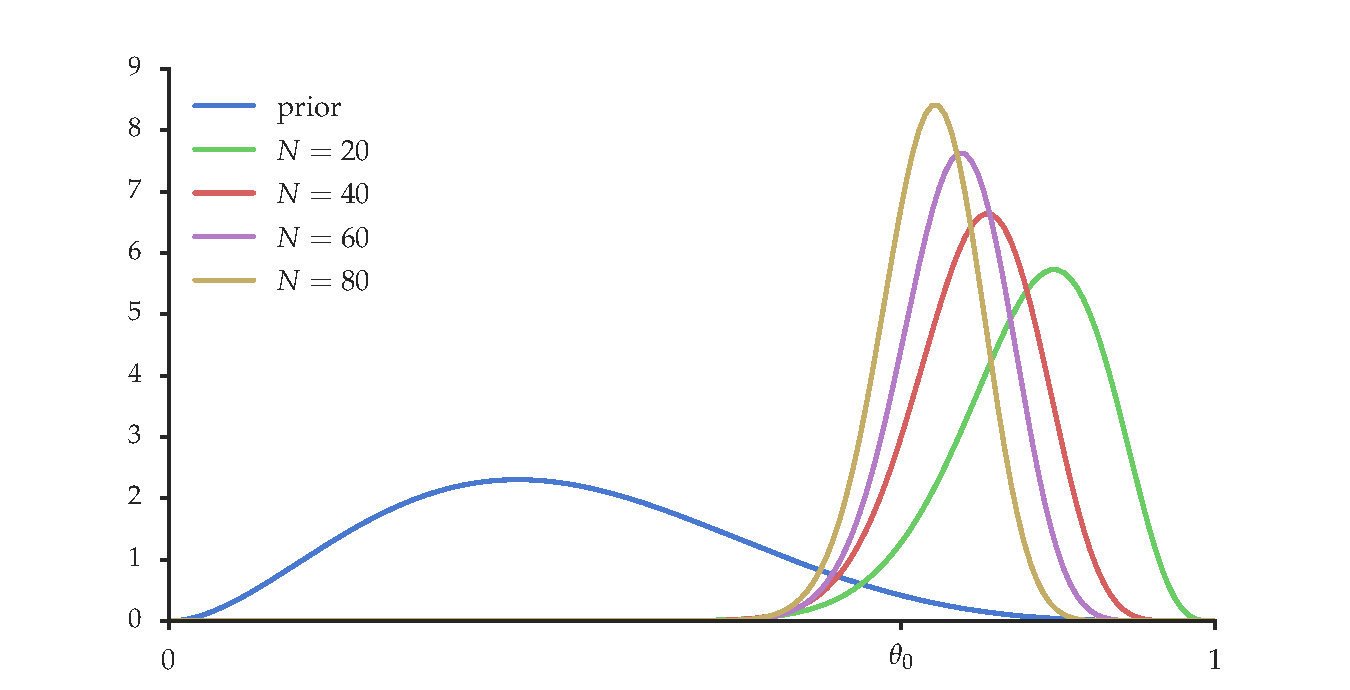
\includegraphics[trim={0em 0em 0em 0em}, clip]{beta_bayes.pdf}}
        \caption{\label{f:beta_bayes} Evolution of the posterior from Beta$(3, 5)$
        prior}
       \end{center}
    \end{figure}

\end{frame}

\begin{frame}

    \vspace{2em}
    Point estimates are extracted from the posterior distribution based on some
    measure of central tendency, such as the mean, the median, or the \navy{mode}
    of the posterior
    
    \vspace{.7em}
    \Eg
        The mean of the posterior in \eqref{eq:betapost2} yields the estimator
        %
        \begin{equation*}
            \hat \theta := \frac{\alpha + x}{\alpha + \beta + N}
        \end{equation*}
        %
        More payouts shift our estimator upwards.  In the limit, $\hat \theta$ is
        near $\frac{x}{N}$, which is the MLE of $\theta$
        
        This illustrates a common theme: difference between maximum likelihood and
        Bayesian estimates typically concerns finite sample properties
        
\end{frame}

\begin{frame}
    
    \vspace{2em}
    Priors where the parametric class is preserved
    under Bayesian updating for a specific likelihood function are called
    \navy{conjugate}
    
    \vspace{.7em}
    In applications, integration over the parameter space carried out
    numerically: standard to use Markov chain Monte Carlo (see \S\ref{ET-ss:mcmc} in ET):
    %
    \begin{itemize}
        \item using MCMC, we can reduce complexity by not having 
        to evaluate the integral in the expression for the posterior distribution
    \end{itemize}
    
\end{frame}

\begin{frame}

    \vspace{2em}
    Popularity of Bayesian methods:
    \begin{enumerate}
        \item  MCMC more successful in practice than 
        the numerical optimization required to obtain maximum likelihood
        estimates
        \item   Bayesian estimation provides a form of
        regularization that stabilizes and typically improves estimation of complex
        models.  See \S\ref{ET-ss:abp} in ET
        \item  Bayesian estimation comes with
        an elegant, unified decision-theoretic approach to inference
    \end{enumerate}
    
\end{frame}

\end{document}
